\chapter{Results}\label{chap:results}

In this chapter, we discuss the results obtained from testing the SafeScript project using different scenarios over the implemented models, namely the GPT API and the LSTM model. 
The primary focus is on the detection of various vulnerabilities such as Cross-Site Scripting (XSS), Command Injection, Path Disclosure, and Remote Code Execution. 
Each case study is analyzed to compare the performance of the GPT API and the LSTM model.

\subsection{Project Pages}

\begin{itemize}
    \item The figure \ref{img:login} shows the login page of the SafeScript.
    \begin{figure}[H]
        \centering
        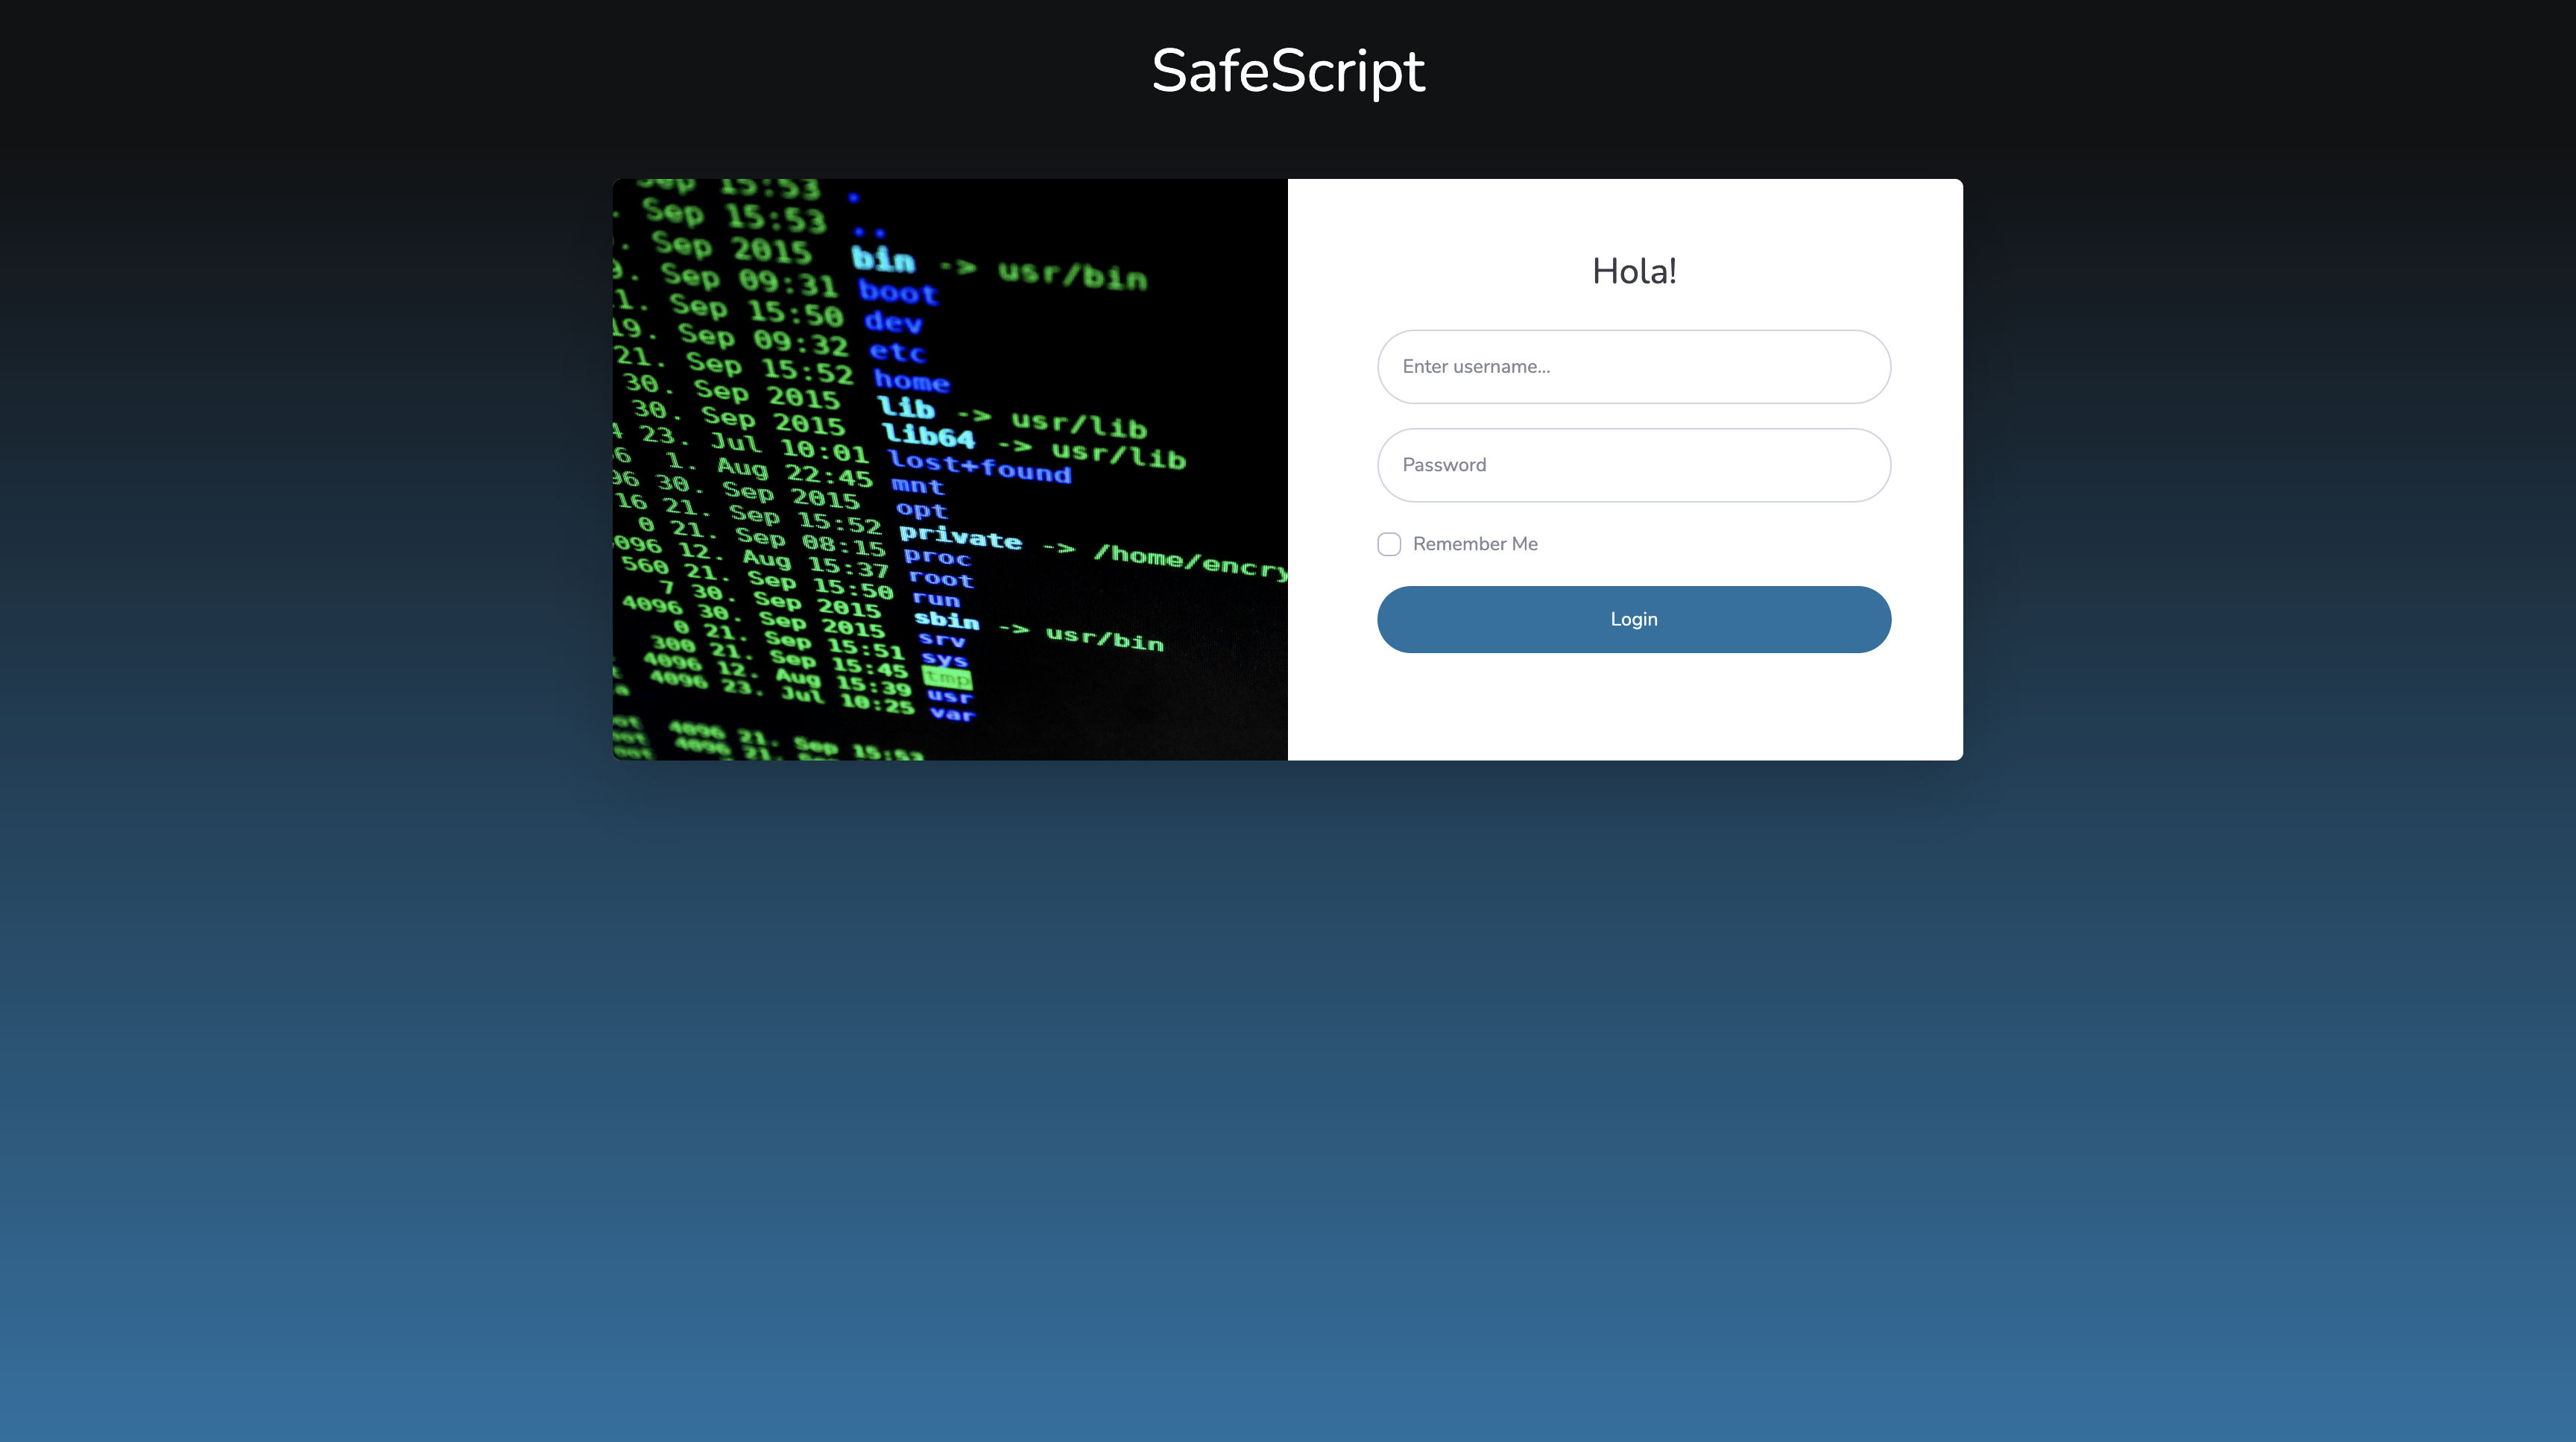
\includegraphics[width=0.6\linewidth]{images/login.png}
        \caption{SafeScript main page}
        \label{img:login}
    \end{figure}
    \item The figure \ref{img:mainpage} shows the main page of the SafeScript.
    \begin{figure}[H]
        \centering
        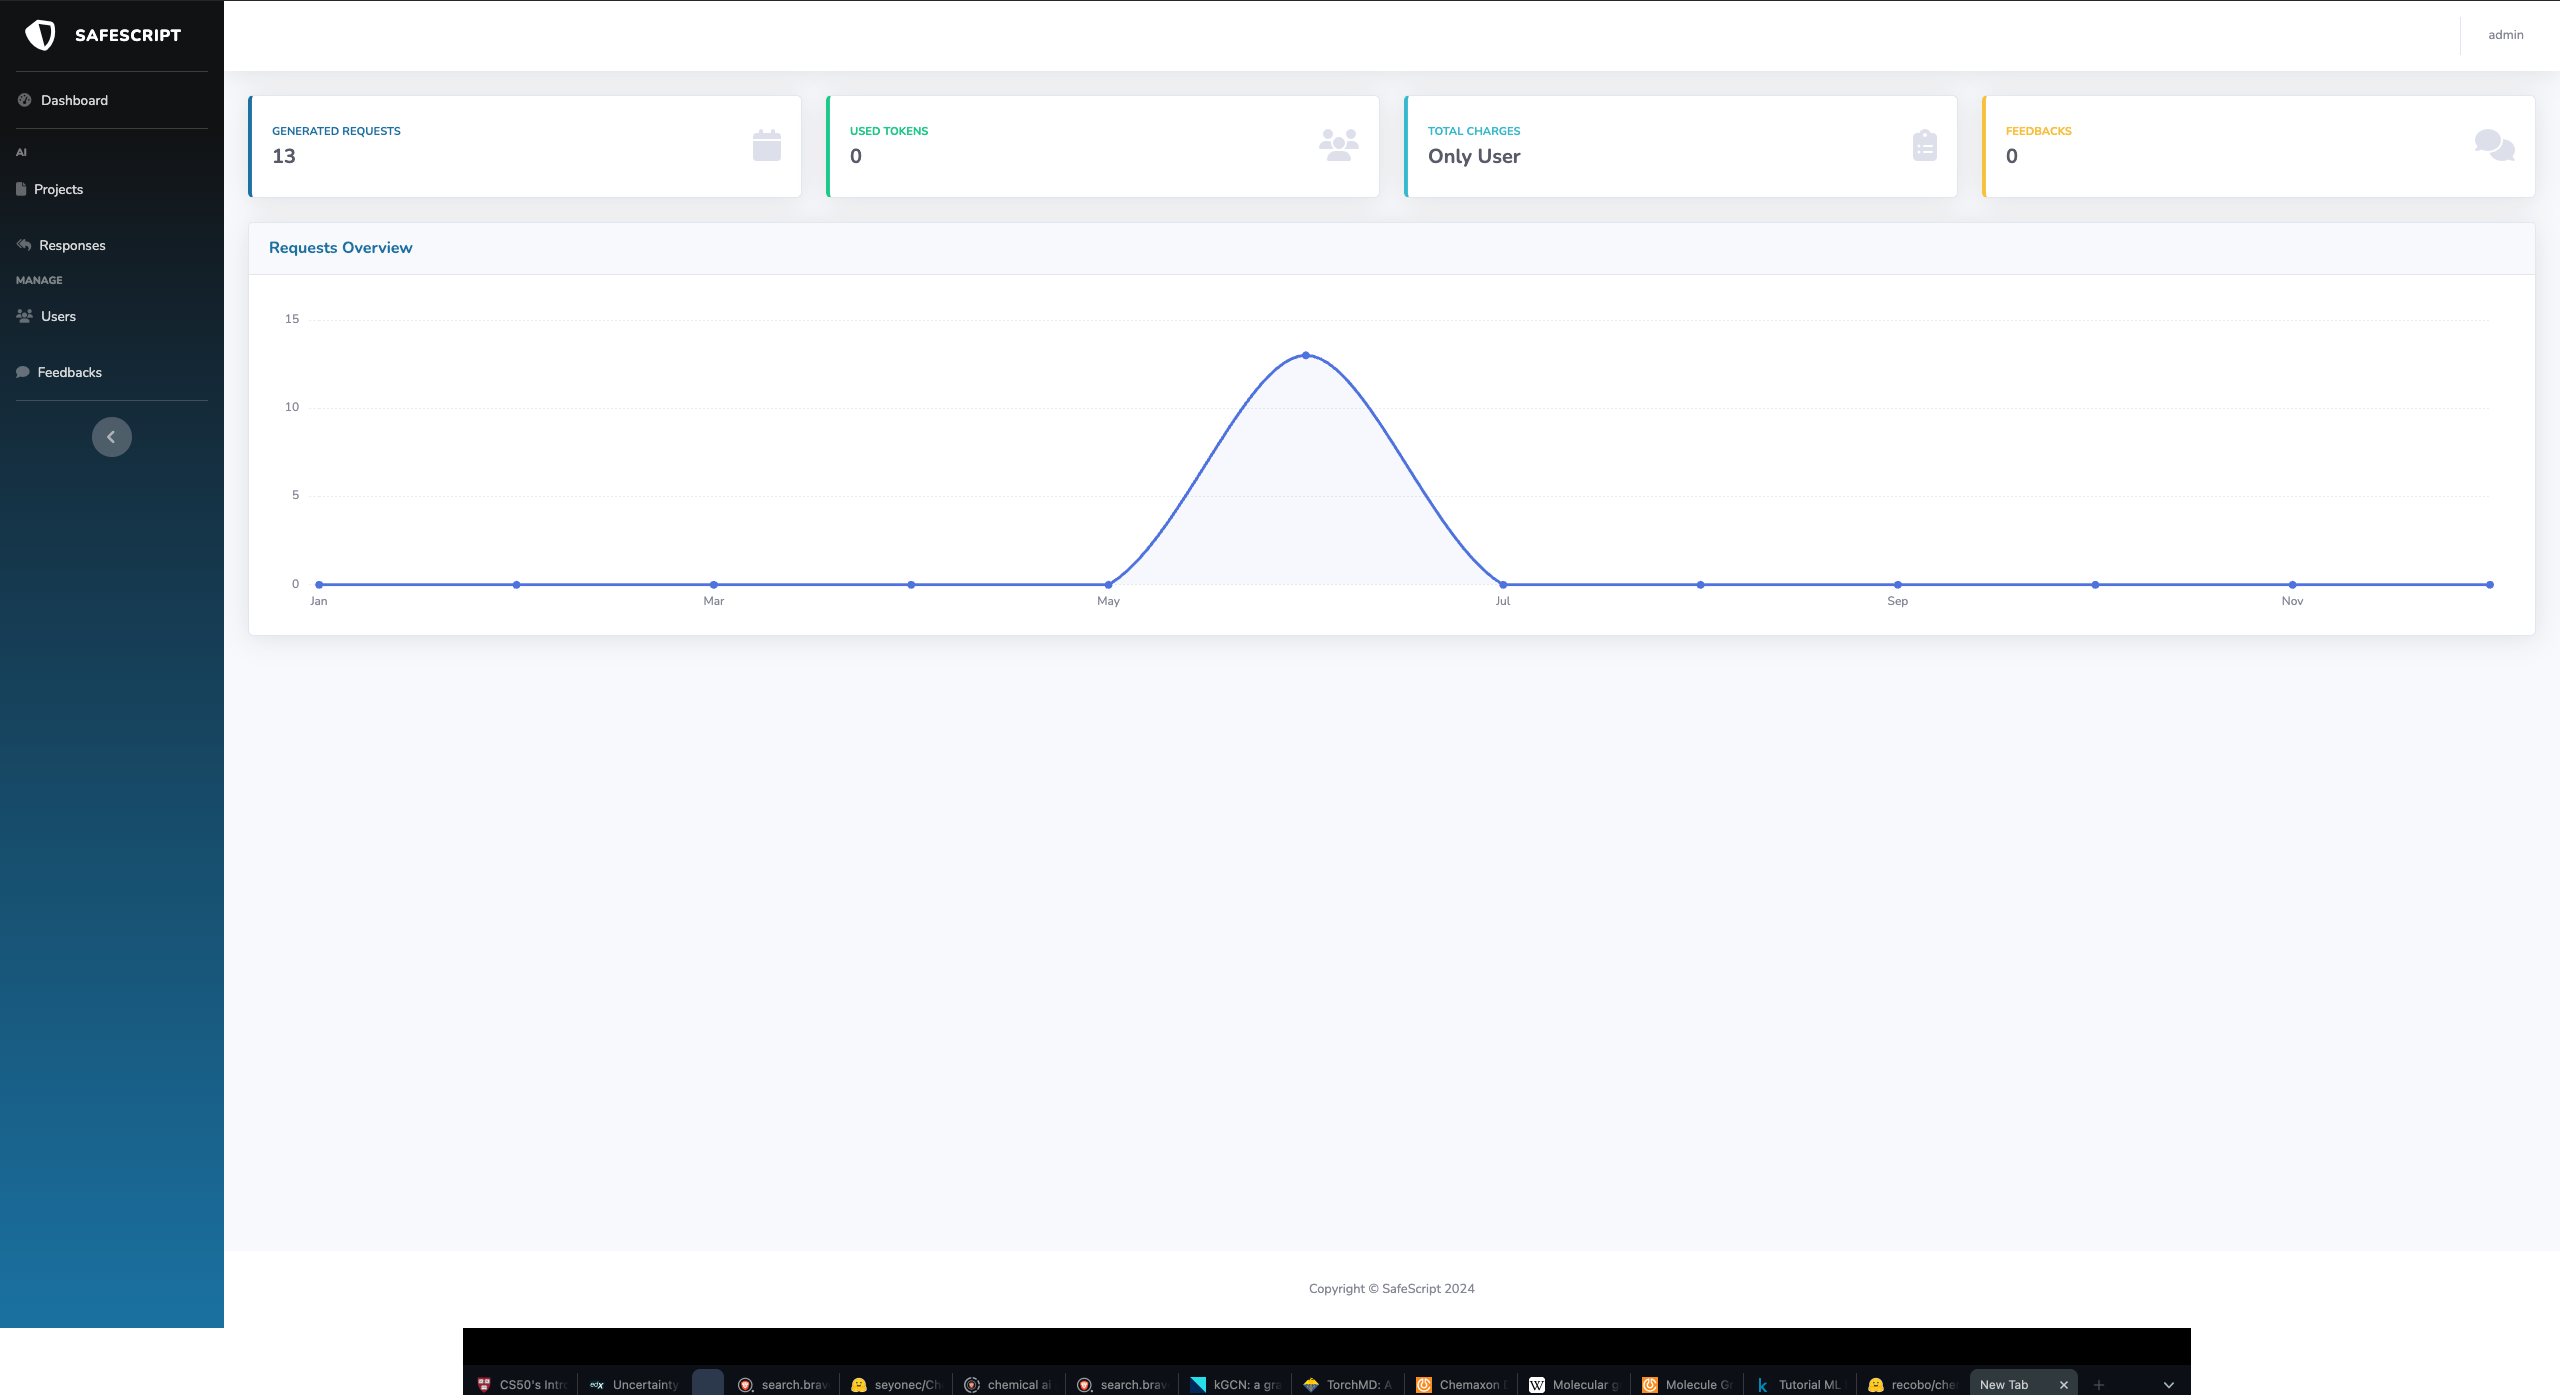
\includegraphics[width=0.6\linewidth]{images/mainpage.png}
        \caption{SafeScript main page}
        \label{img:mainpage}
    \end{figure}
    \item The figure \ref{img:project} shows the projects page of the SafeScript.
    \begin{figure}[H]
        \centering
        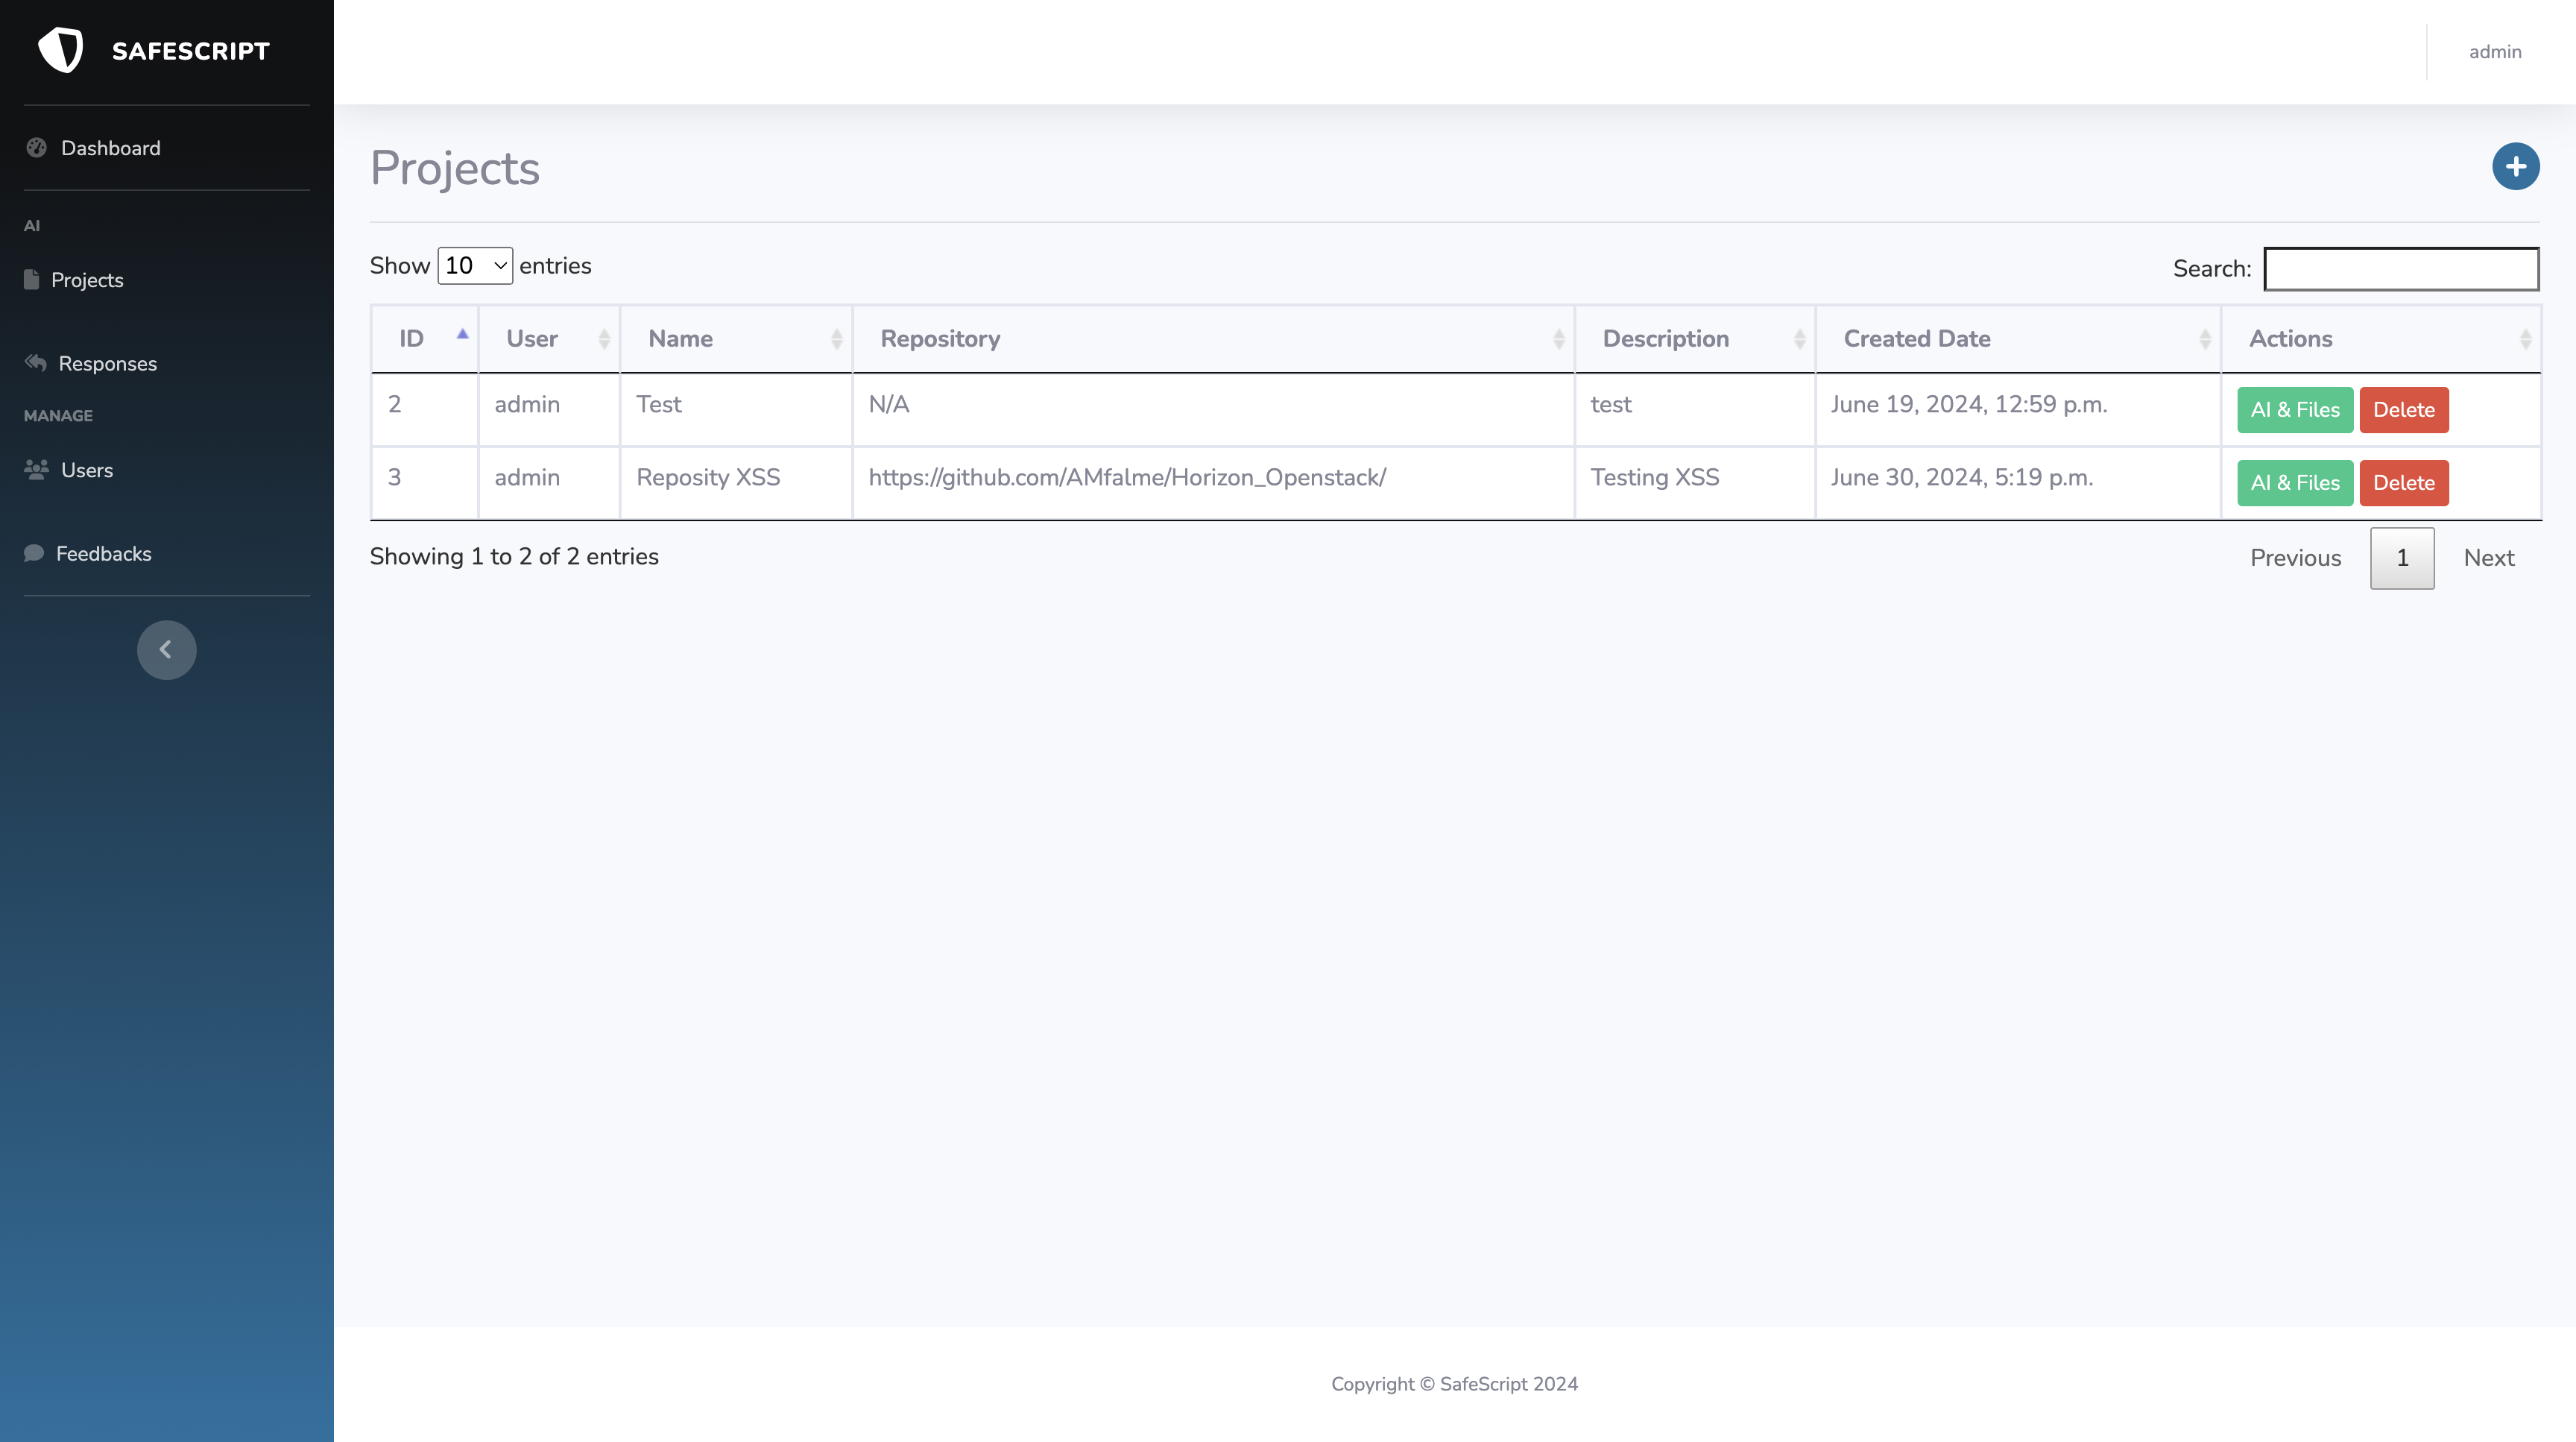
\includegraphics[width=0.6\linewidth]{images/projects.png}
        \caption{SafeScript projects page}
        \label{img:project}
    \end{figure}
    \item The figure \ref{img:users} shows users of the SafeScript.
    \begin{figure}[H]
        \centering
        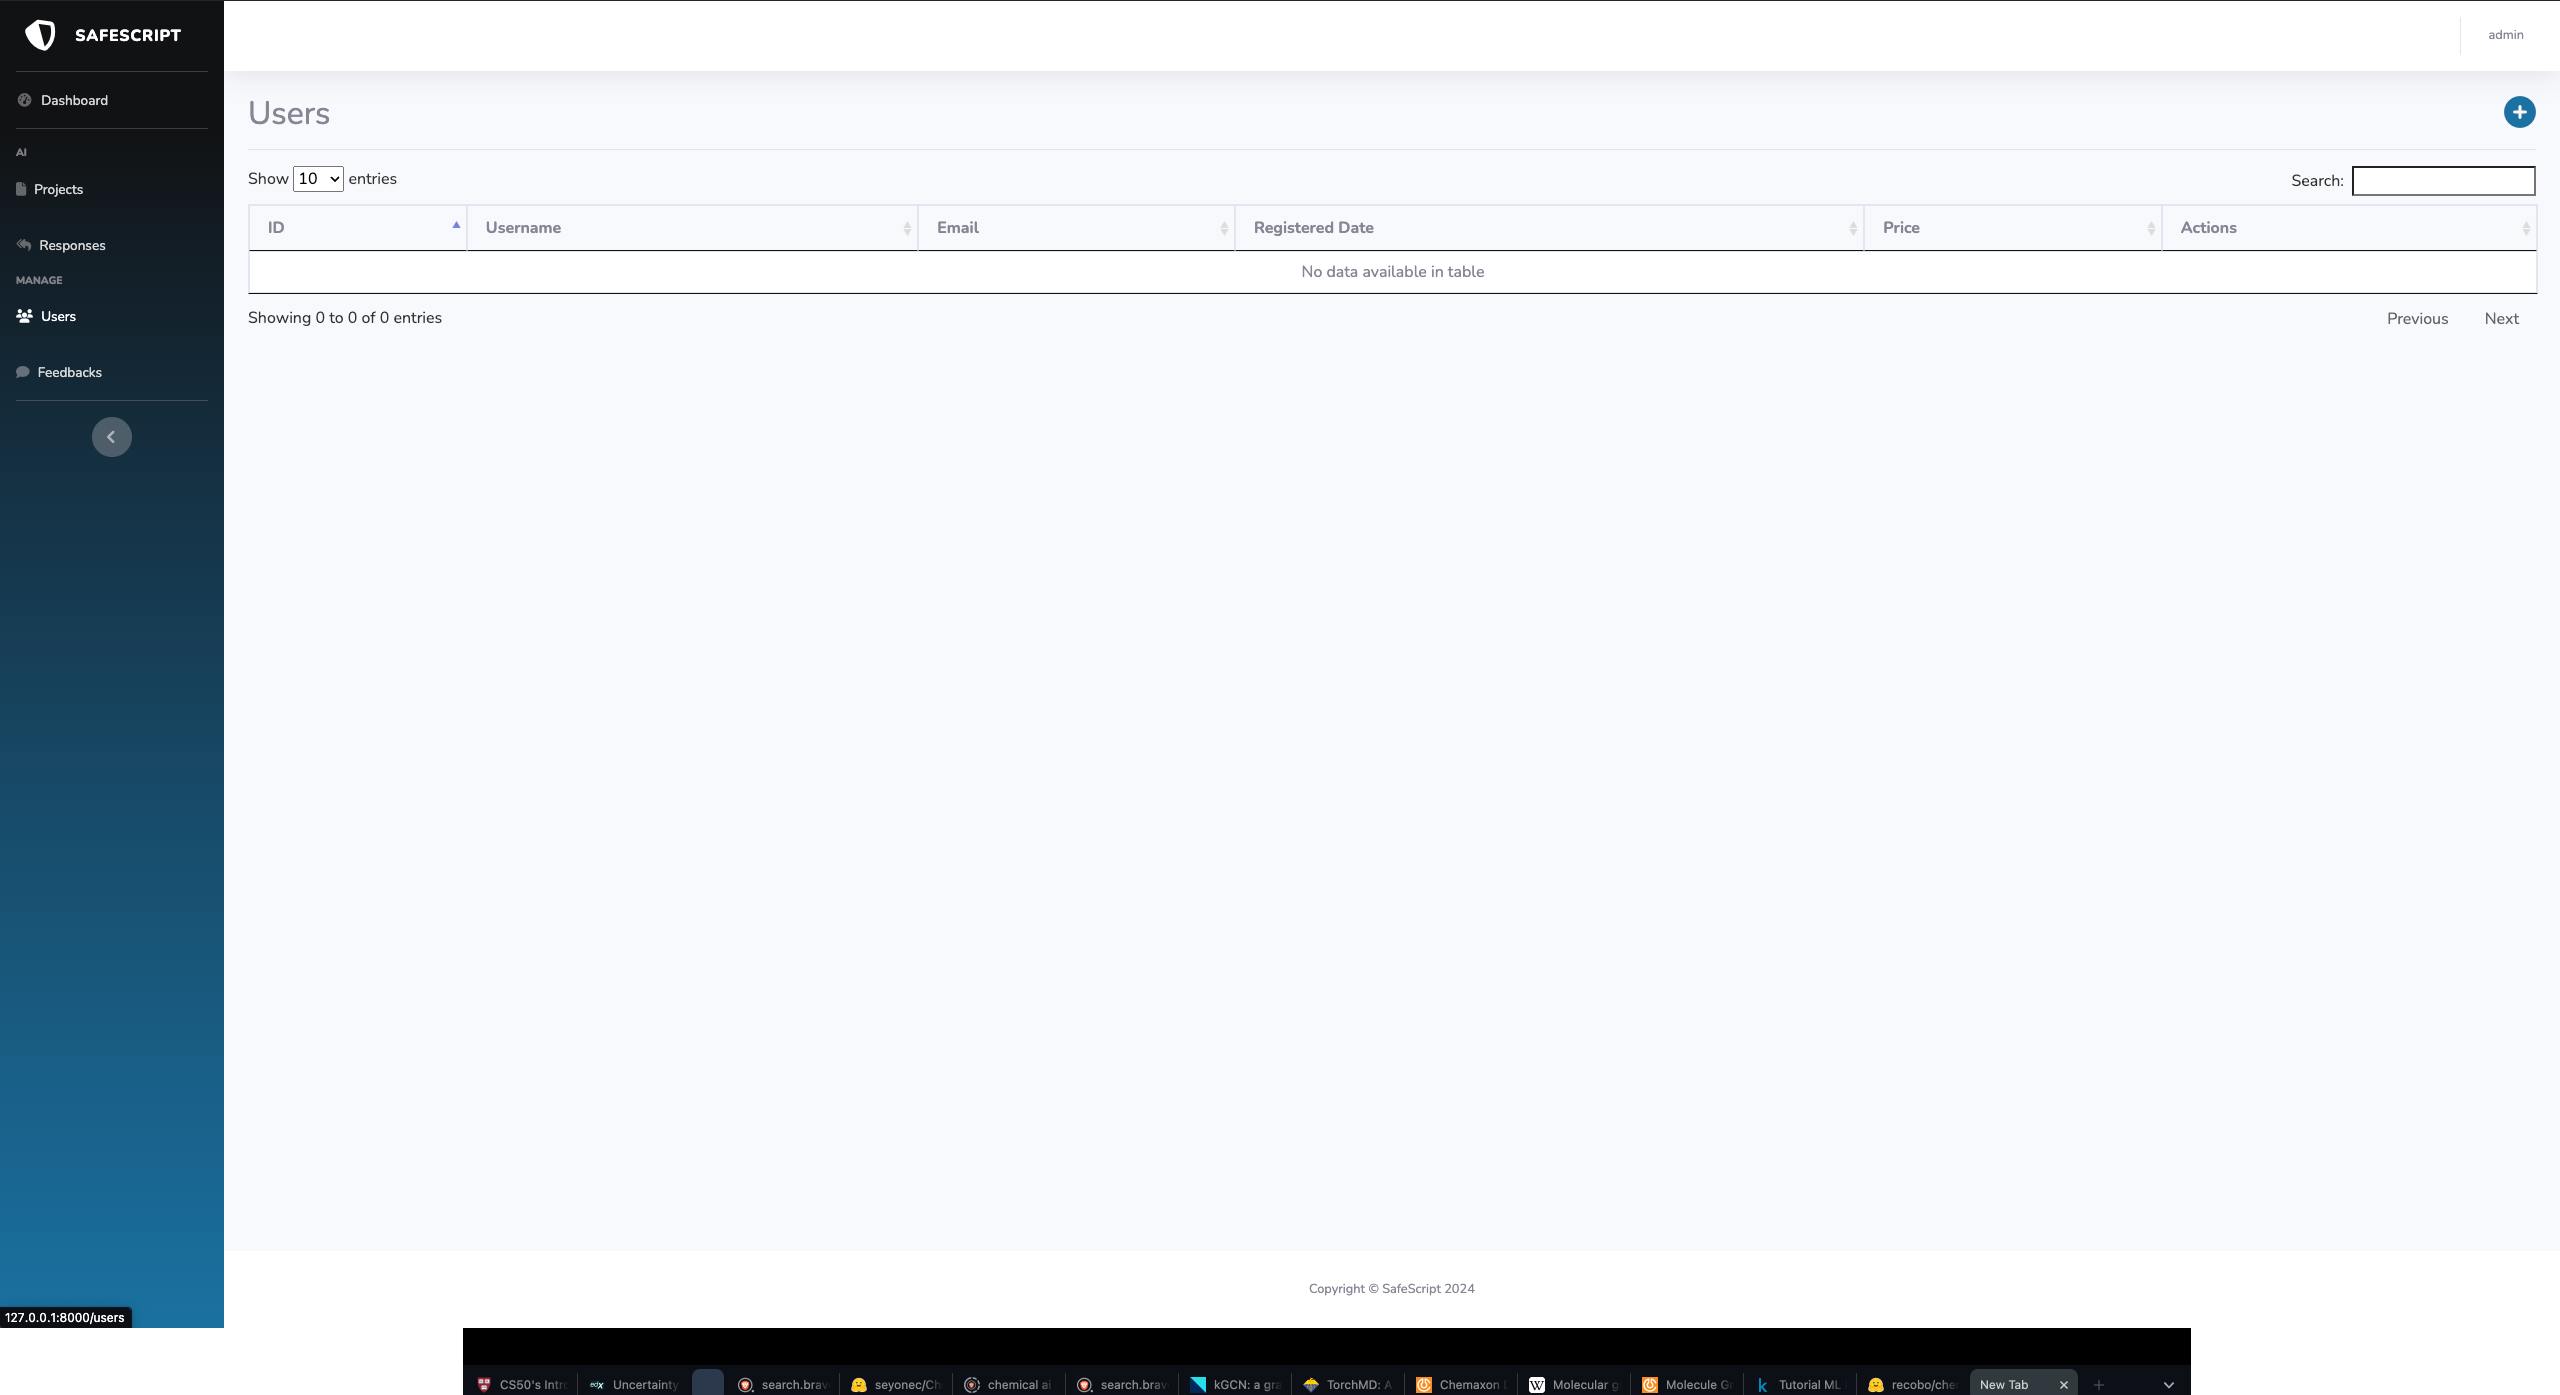
\includegraphics[width=0.6\linewidth]{images/users.png}
        \caption{SafeScript users page}
        \label{img:users}
    \end{figure}
    \item The figure \ref{img:feedback} shows feedback page of the SafeScript.
    \begin{figure}[H]
        \centering
        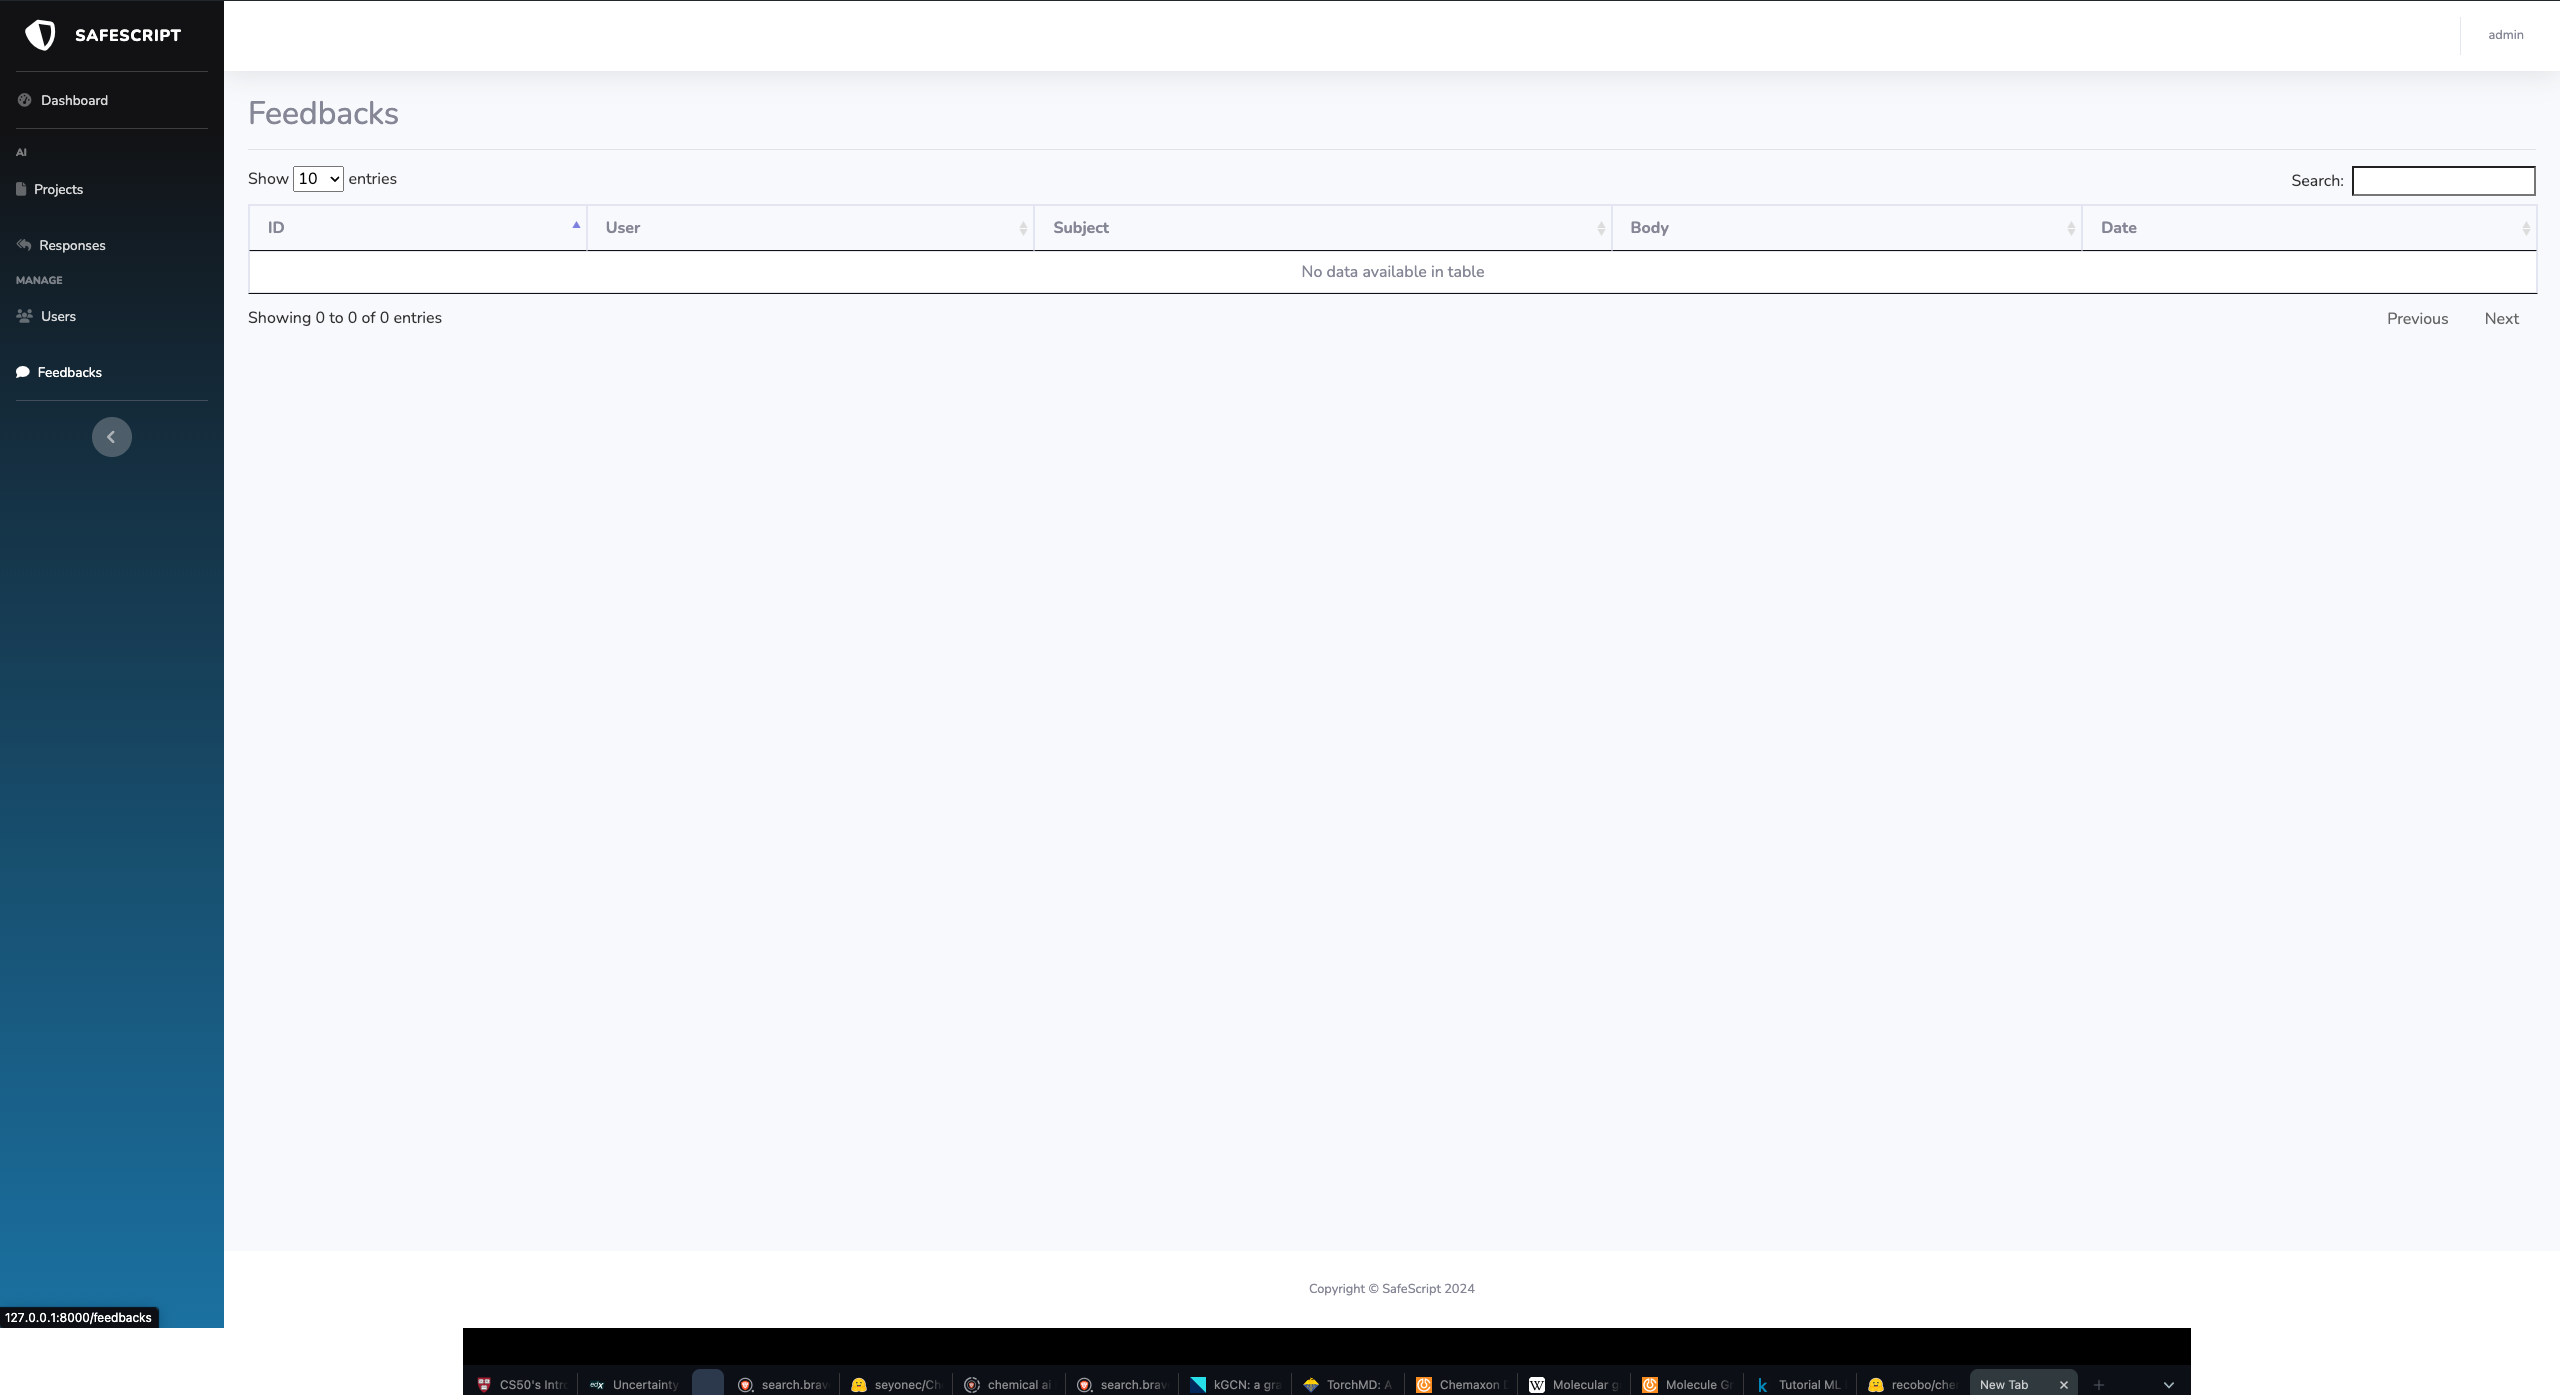
\includegraphics[width=0.6\linewidth]{images/feedback.png}
        \caption{SafeScript feedback page}
        \label{img:feedback}
    \end{figure}


\end{itemize}

\subsection{GPT API}
In Below there are two test cases that have been tested over GPT API.

\begin{itemize}
    \item The figure \ref{img:skey_gpt} shows testing of Skey script over GPT API.
    \begin{figure}[H]
        \centering
        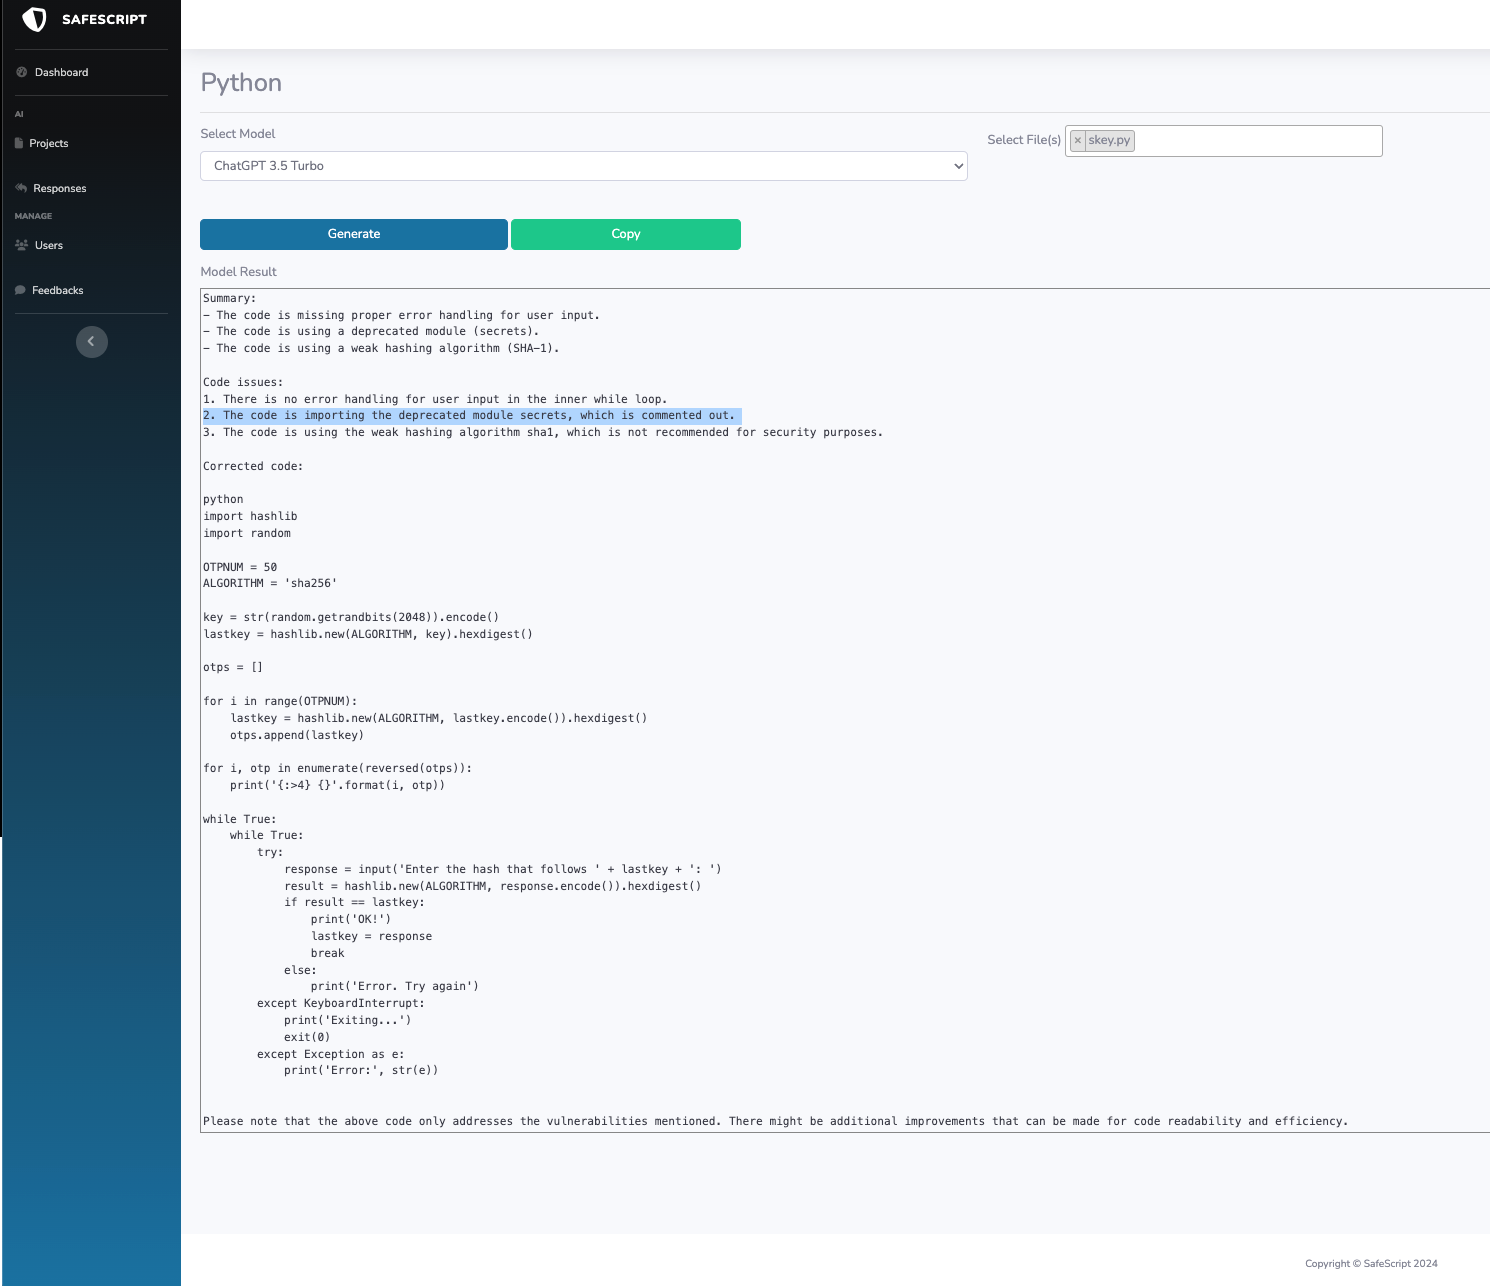
\includegraphics[width=0.6\linewidth]{images/skey_gpt.png}
        \caption{Testing Skey script over GPT}
        \label{img:skey_gpt}
    \end{figure}

    \item The figure \ref{img:vulpy_gpt} shows testing of vulpy script over GPT API.
    \begin{figure}[H]
        \centering
        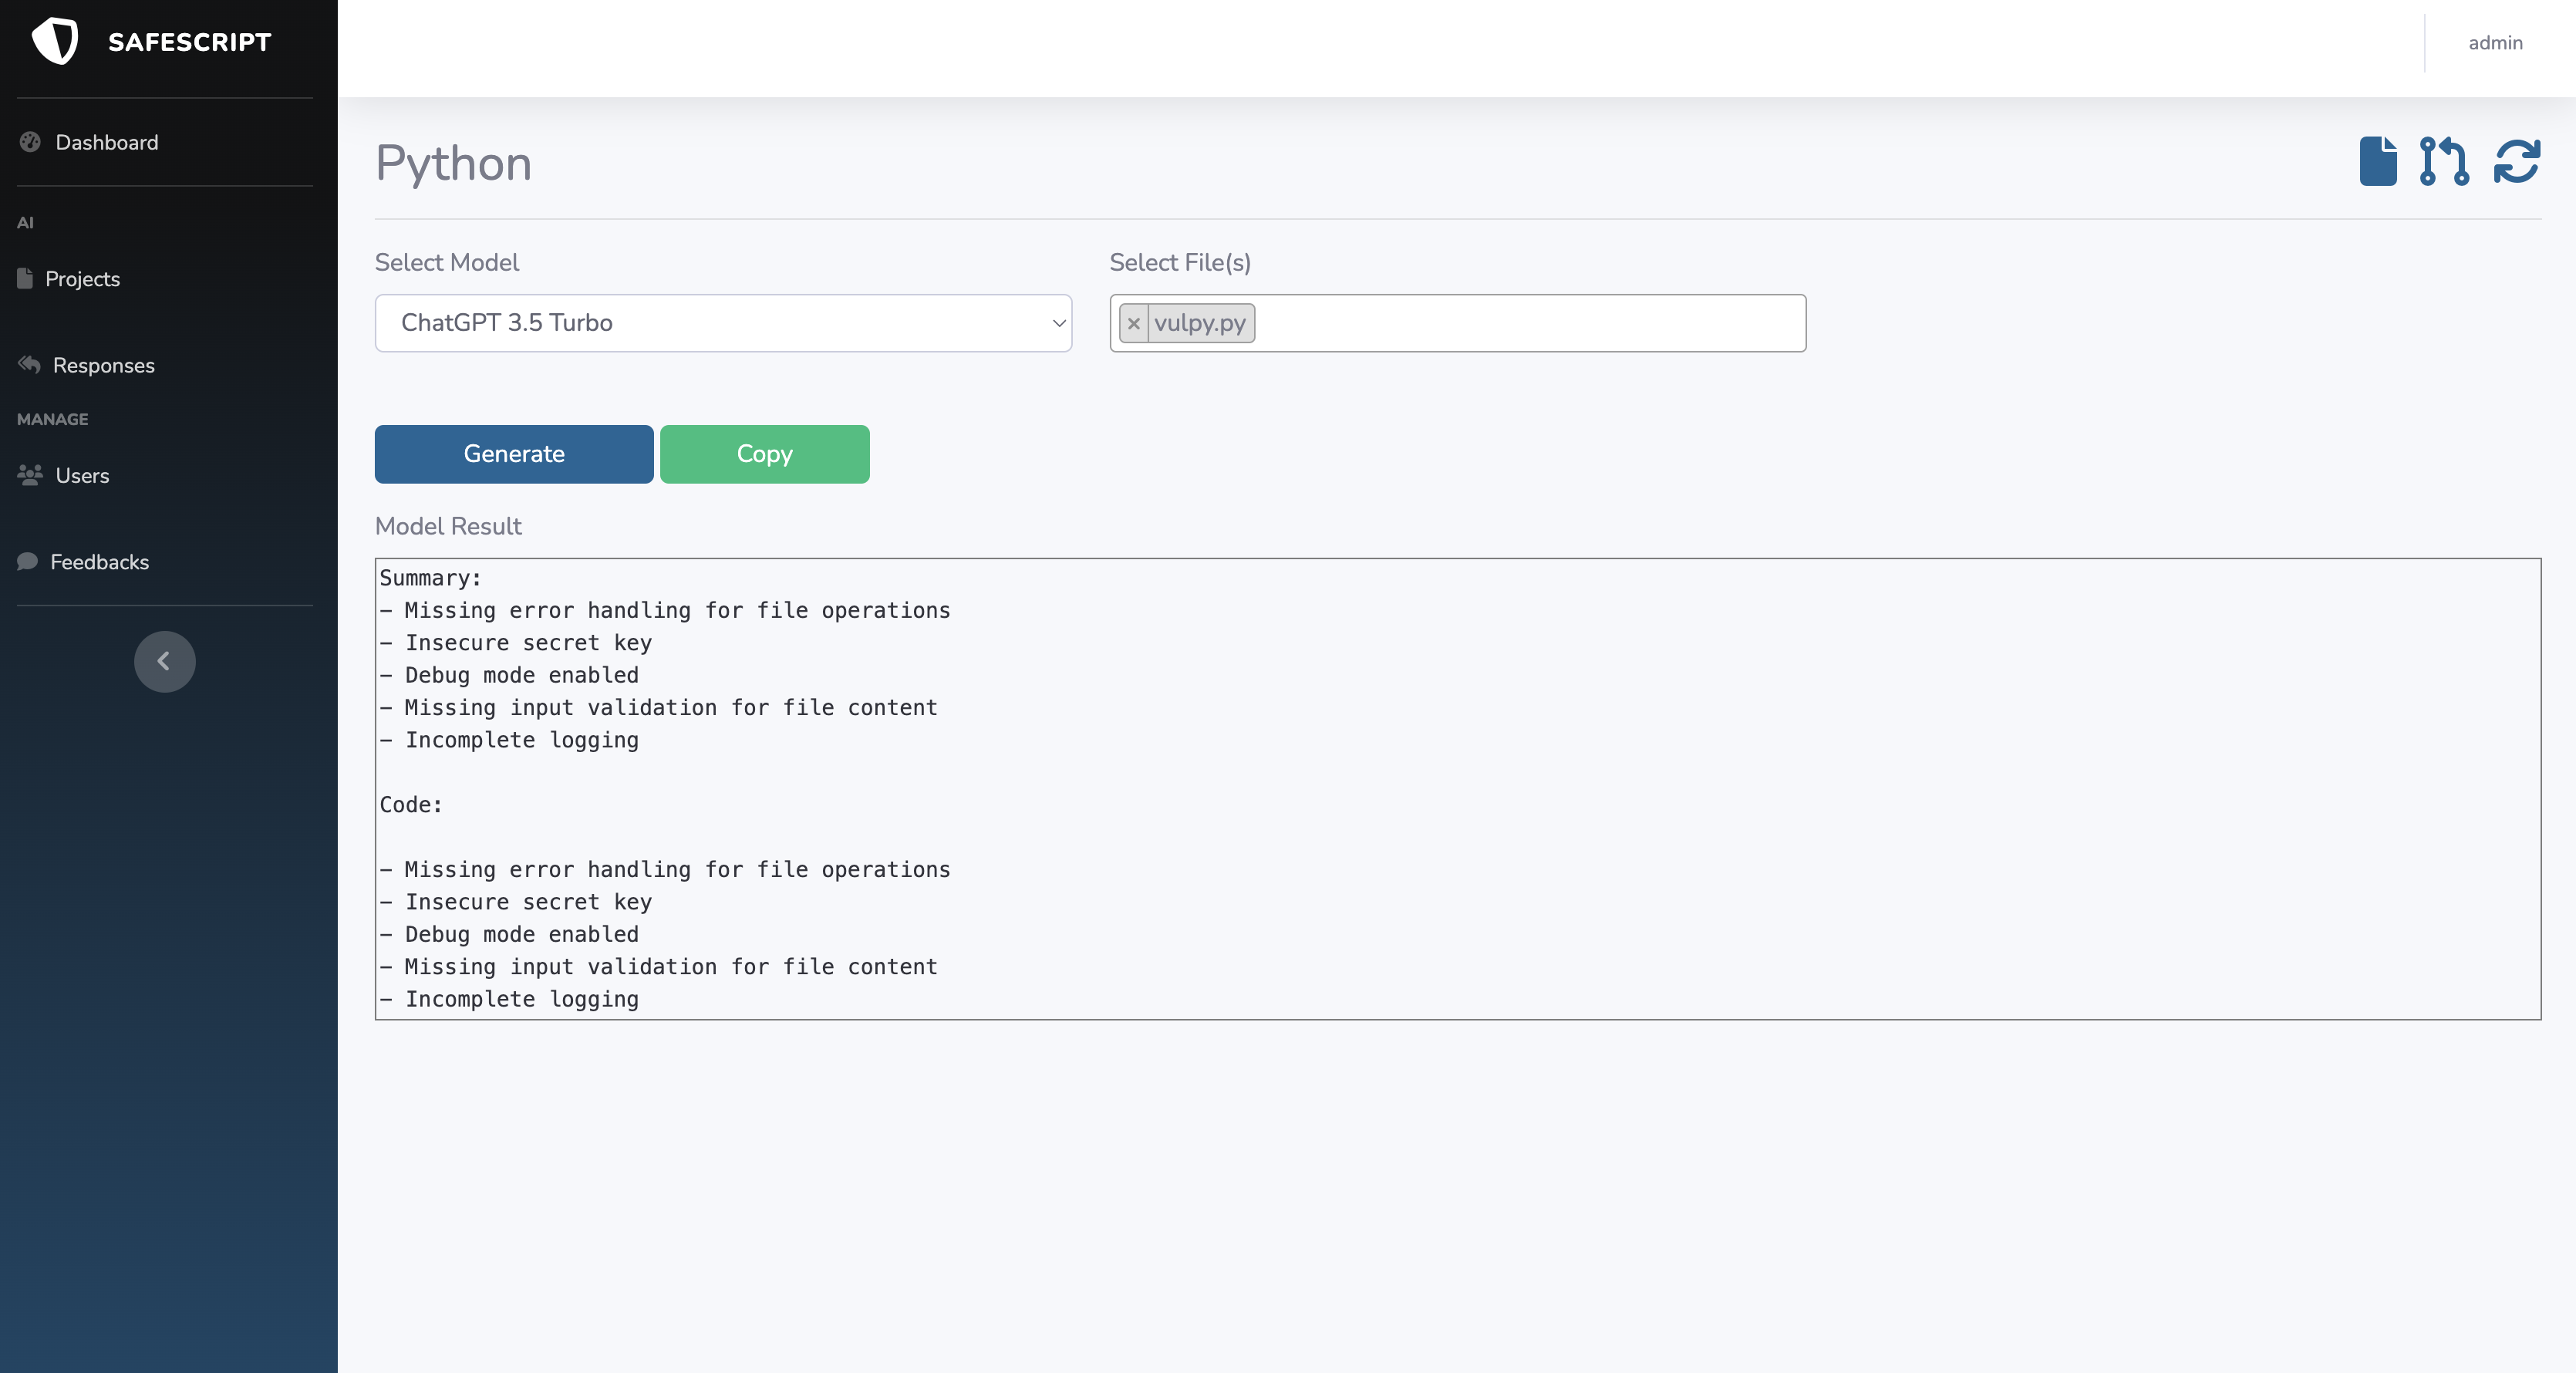
\includegraphics[width=0.6\linewidth]{images/vulpy_gpt.png}
        \caption{Testing Vulpy script over GPT}
        \label{img:vulpy_gpt}
    \end{figure}

\end{itemize}


\subsection{LSTM}
\subsubsection{Reposities}
\begin{itemize}
    \item The figure \ref{img:lstmrepoxss} shows simple program from Mod\_Posts.
    \begin{figure}[H]
        \centering
        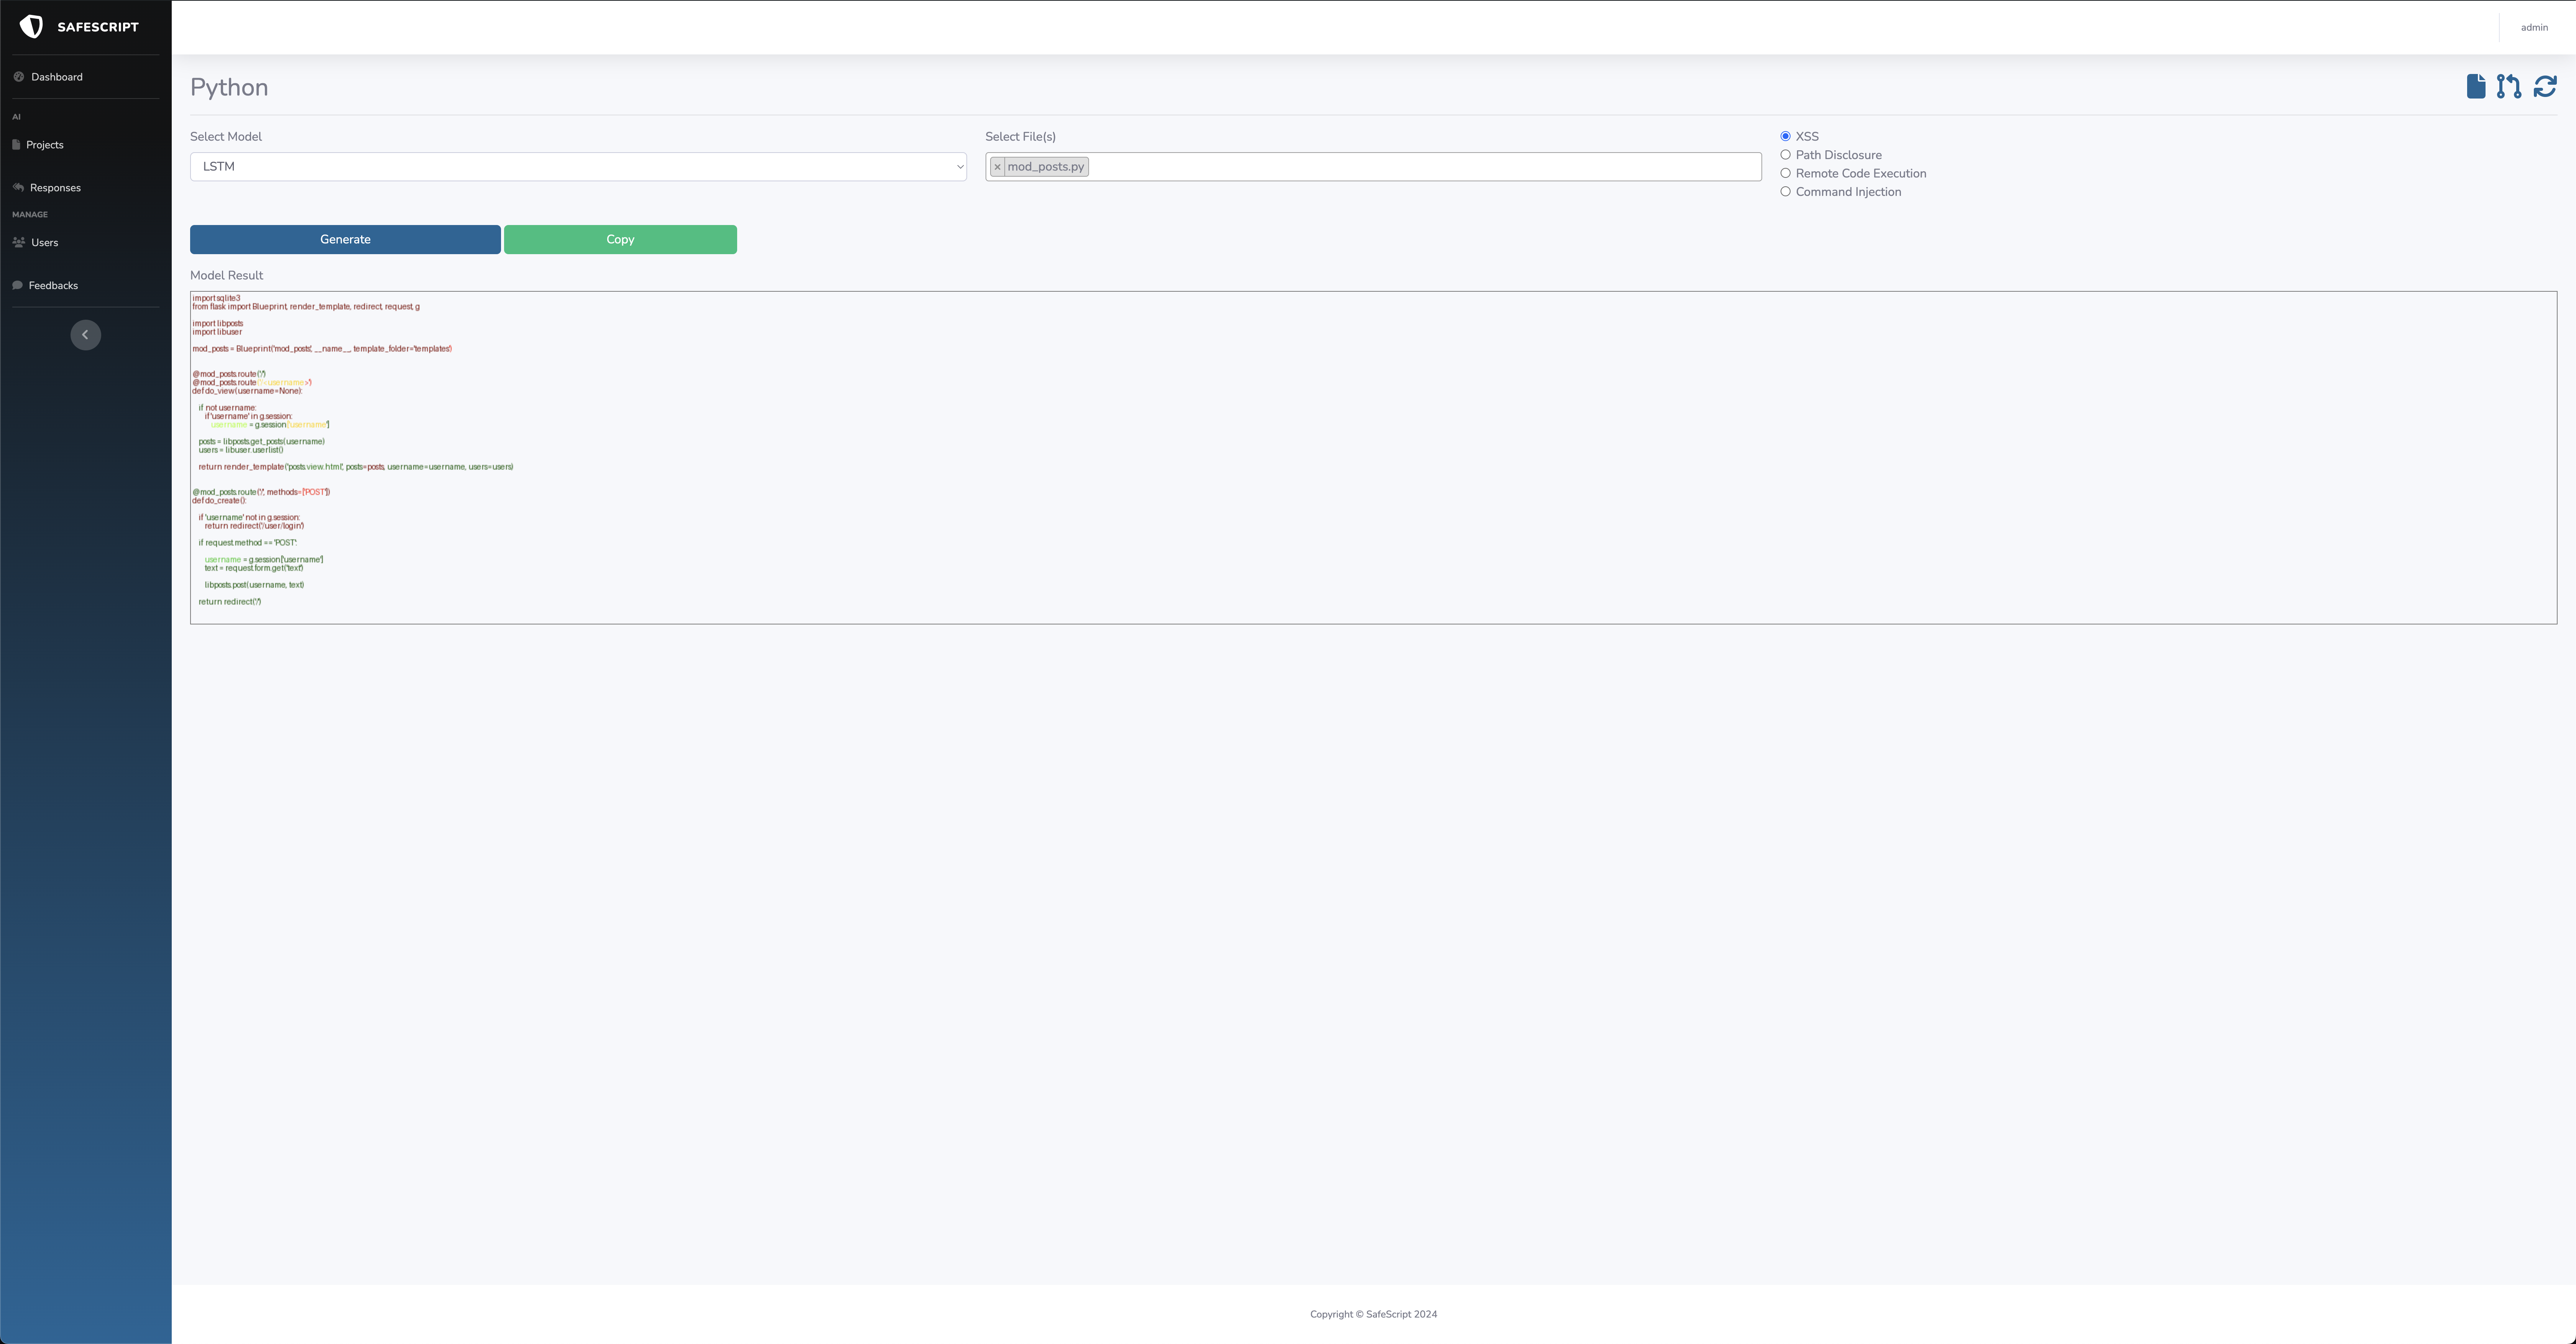
\includegraphics[width=0.6\linewidth]{images/lstm-repo-xss.png}
        \caption{Testing XSS vulnerability over LSTM model with Repository option}
        \label{img:lstmrepoxss}
    \end{figure}

    \item The figure \ref{img:lstmrepopd} shows simple program from Mod\_Posts \cite{vulpy}.
    \begin{figure}[H]
        \centering
        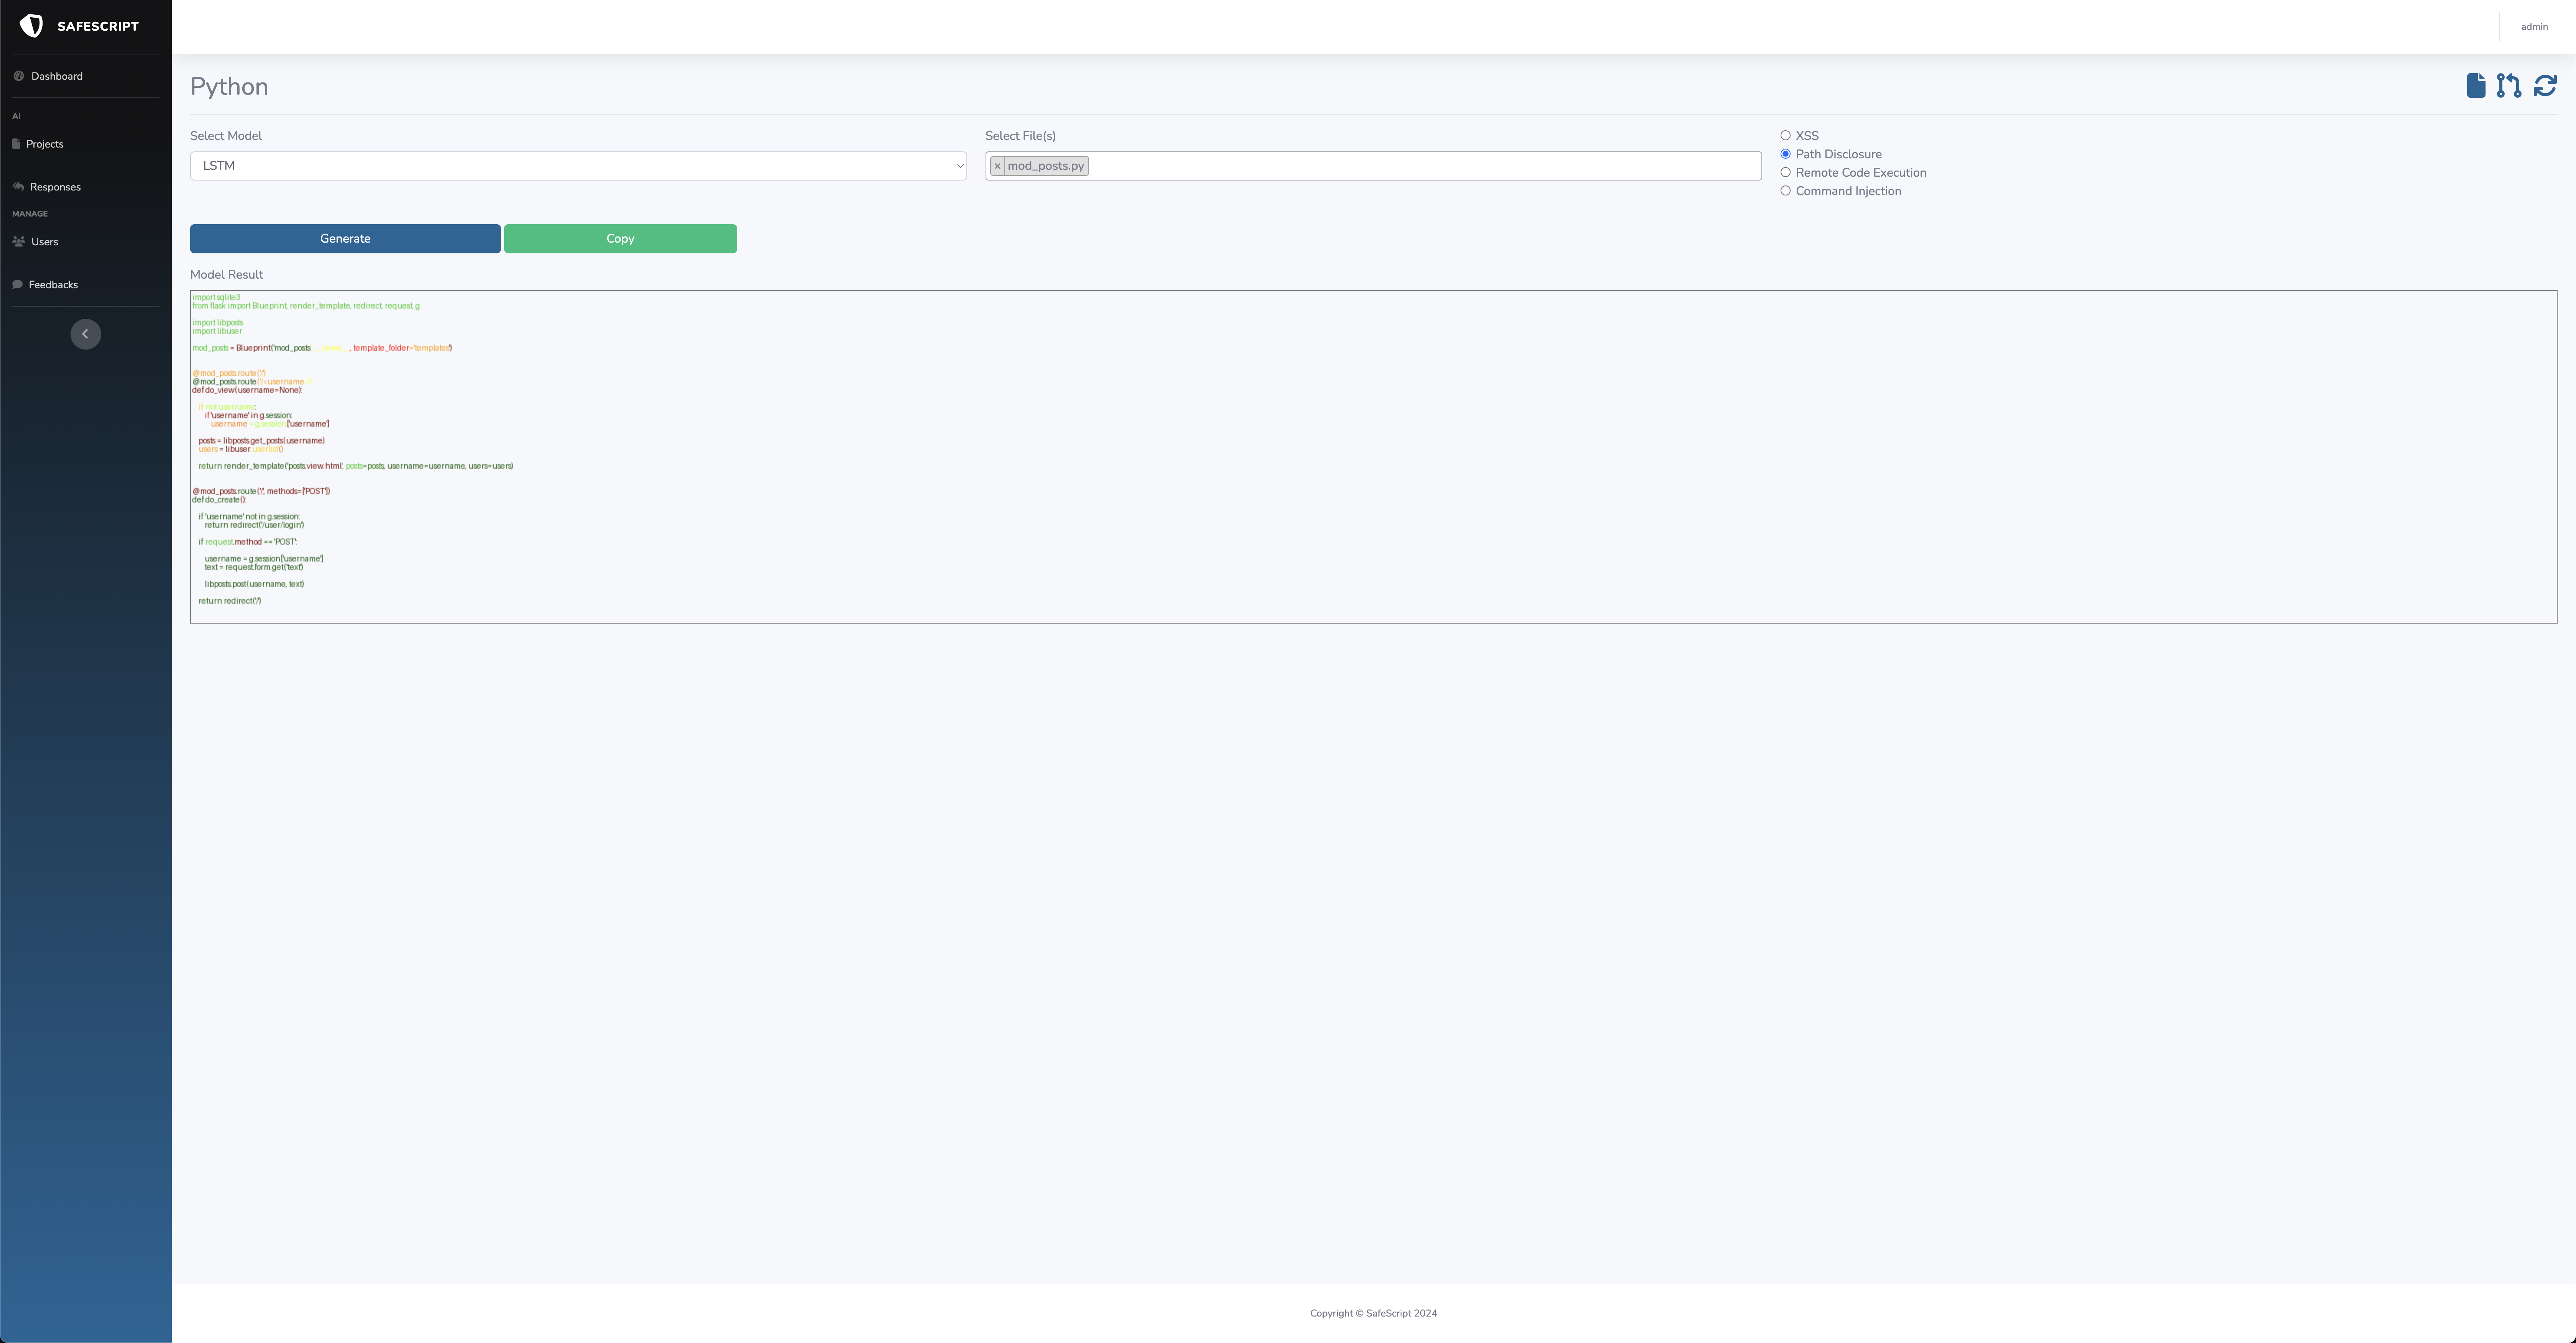
\includegraphics[width=0.6\linewidth]{images/lstm-repo-pd.png}
        \caption{Testing Path Disclosure vulnerability over LSTM model with Repository option}
        \label{img:lstmrepopd}
    \end{figure}

    \item First case: The figure \ref{img:lstmrepoci} shows simple program from Mod\_Posts.
    \begin{figure}[H]
        \centering
        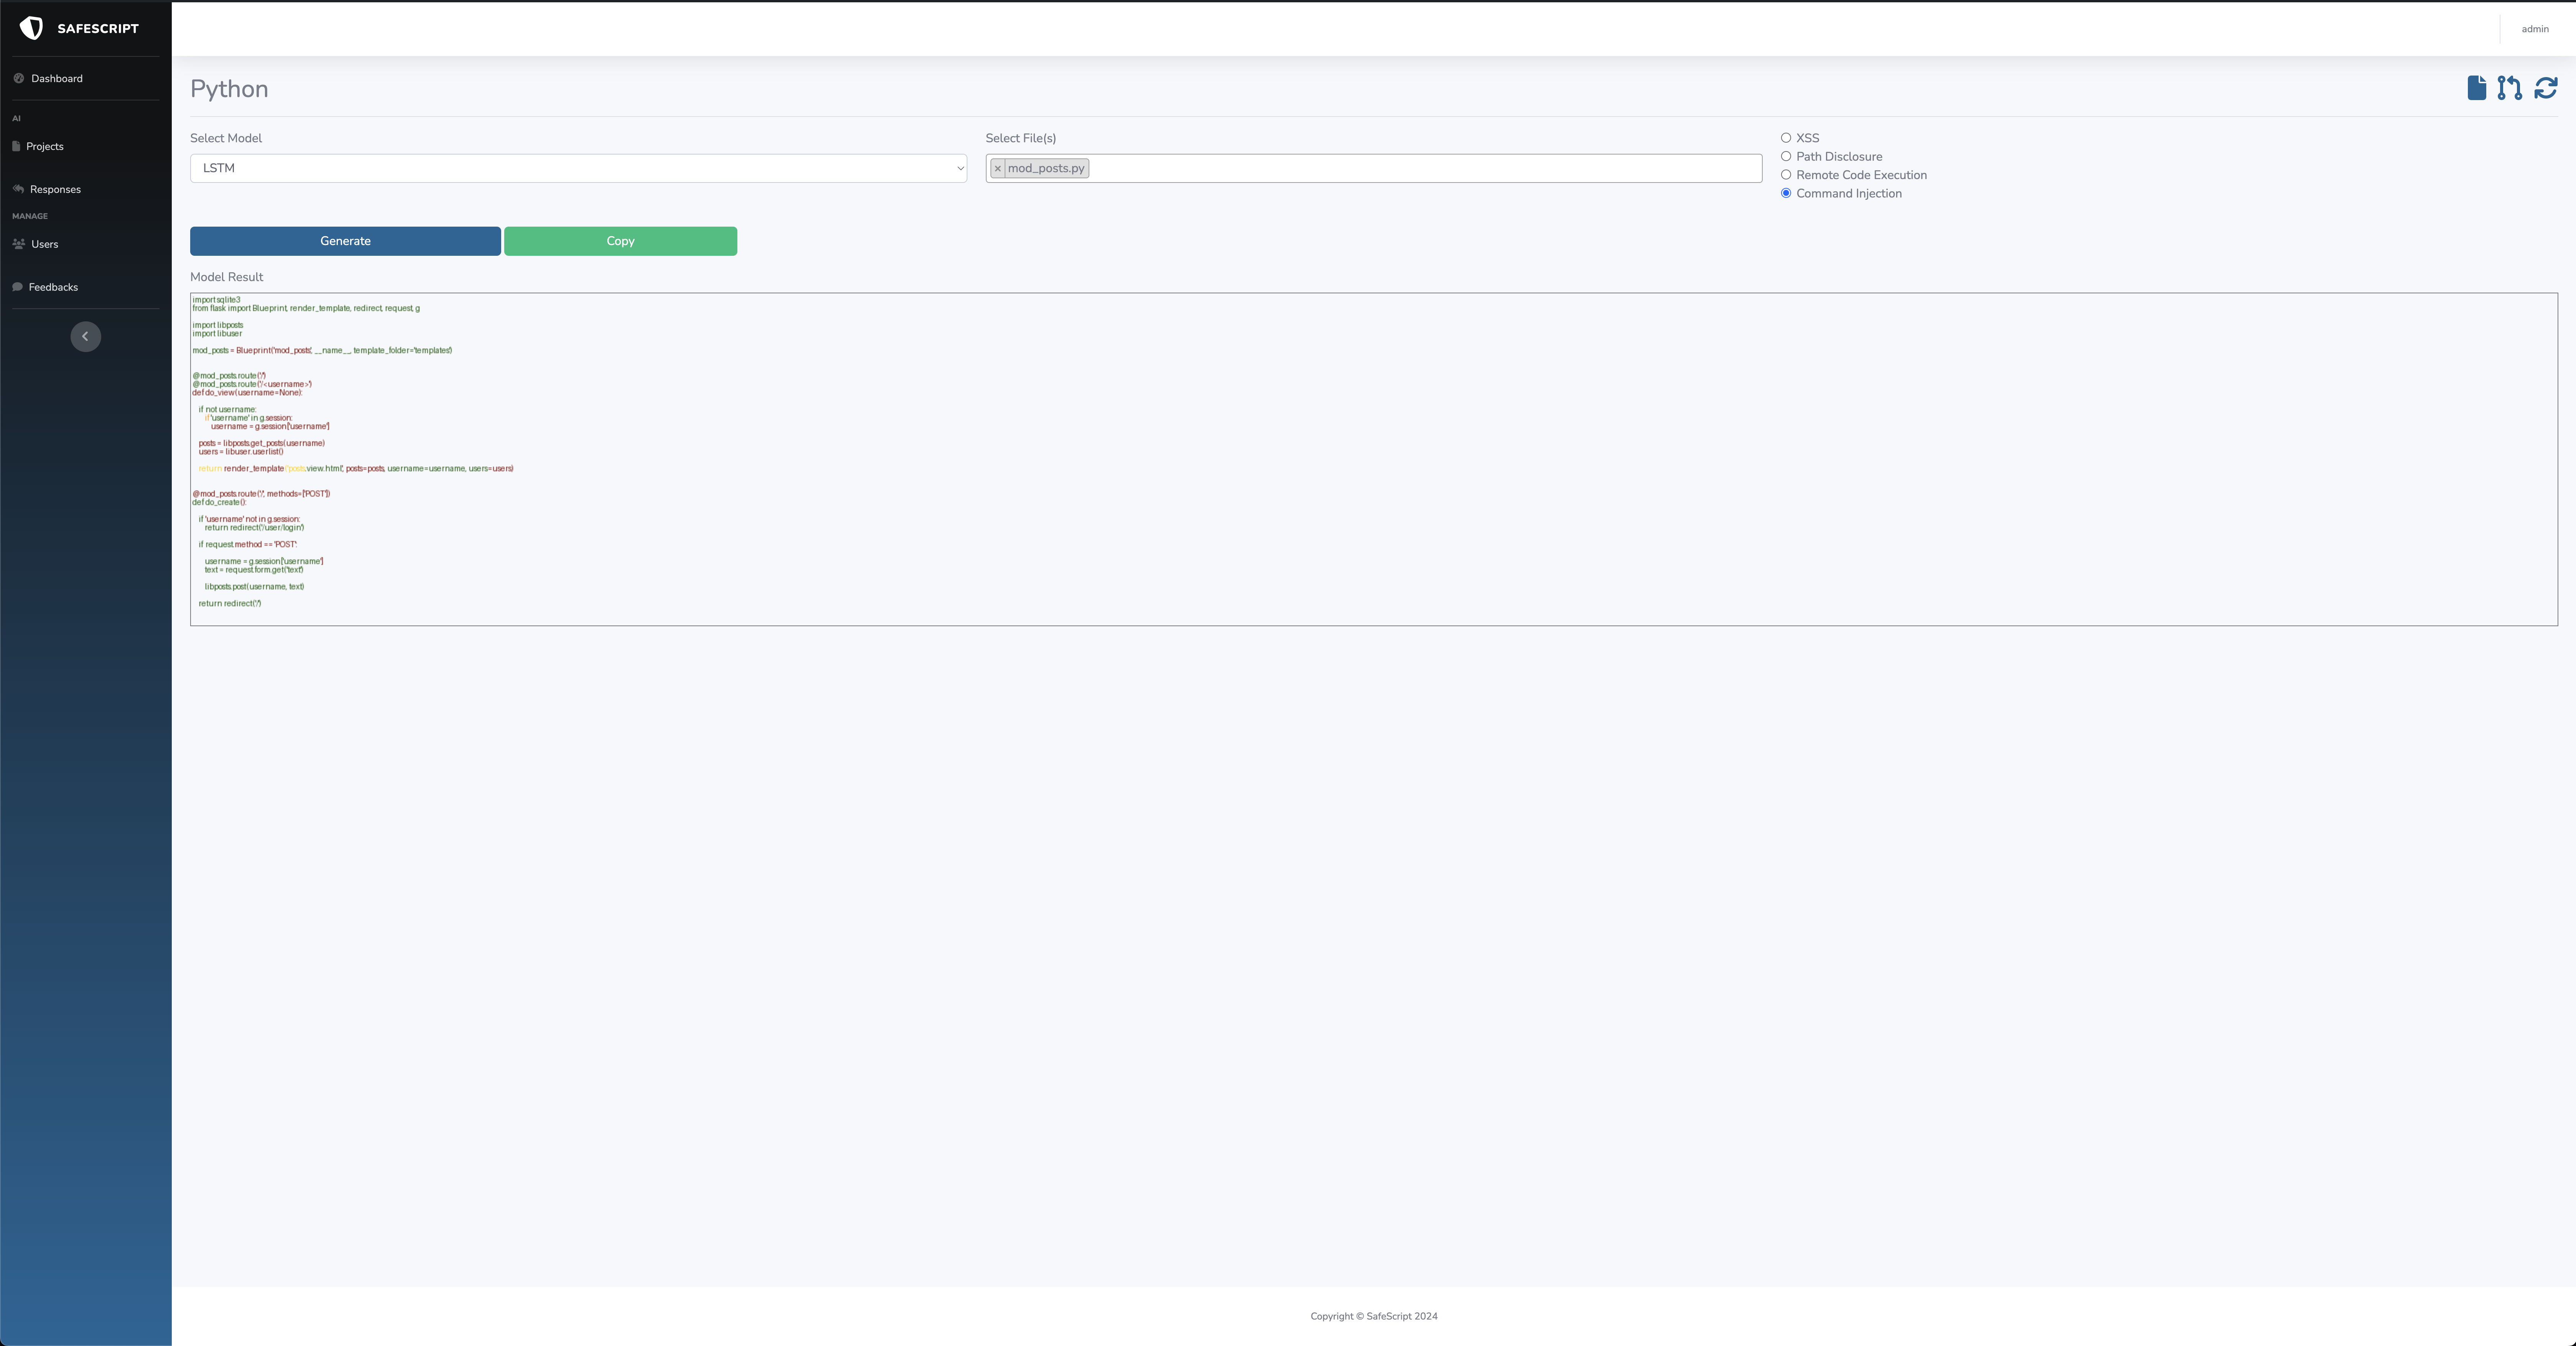
\includegraphics[width=0.6\linewidth]{images/lstm-repo-ci.png}
        \caption{Testing Command Injection vulnerability over LSTM model with Repository option}
        \label{img:lstmrepoci}
    \end{figure}

    \item First case: The figure \ref{img:lstmreporce} shows simple program from Mod\_Posts.
    \begin{figure}[H]
        \centering
        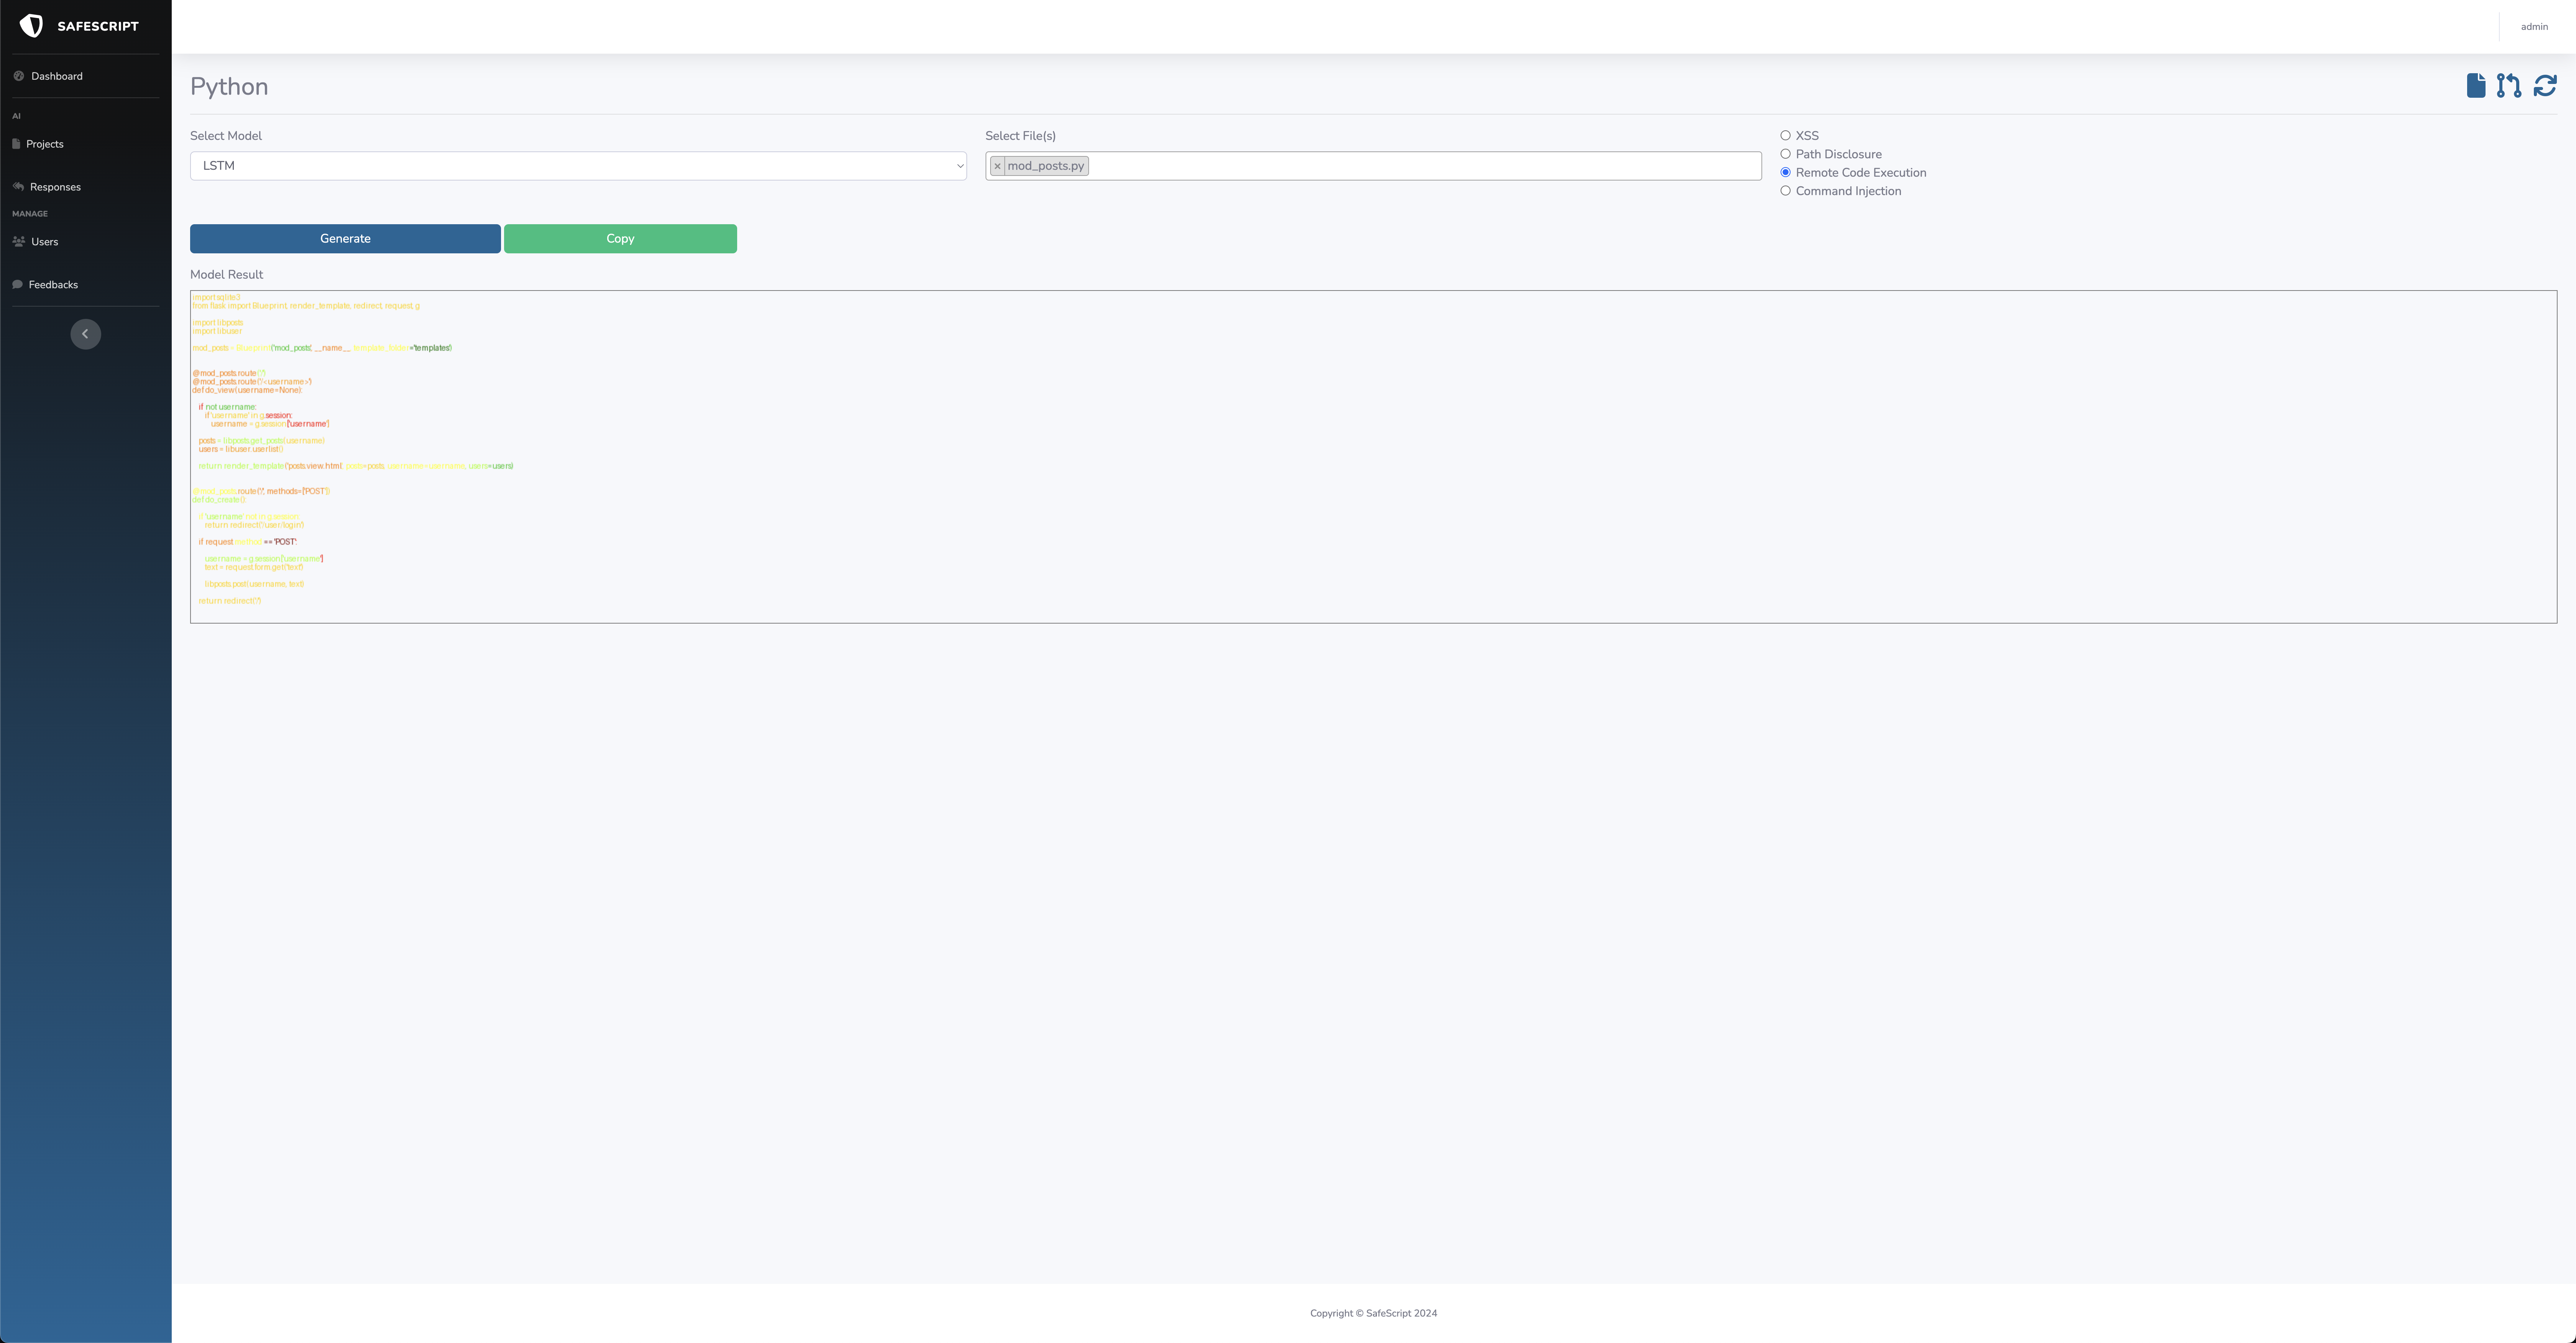
\includegraphics[width=0.6\linewidth]{images/lstm-repo-rce.png}
        \caption{Testing Remote Code Execution vulnerability over LSTM model with Repository option}
        \label{img:lstmreporce}
    \end{figure}
\end{itemize}
\subsubsection{Single file}

\begin{itemize}
    \item First case: The figure \ref{img:xss1} shows simple program from Flask.
    \begin{figure}[H]
        \centering
        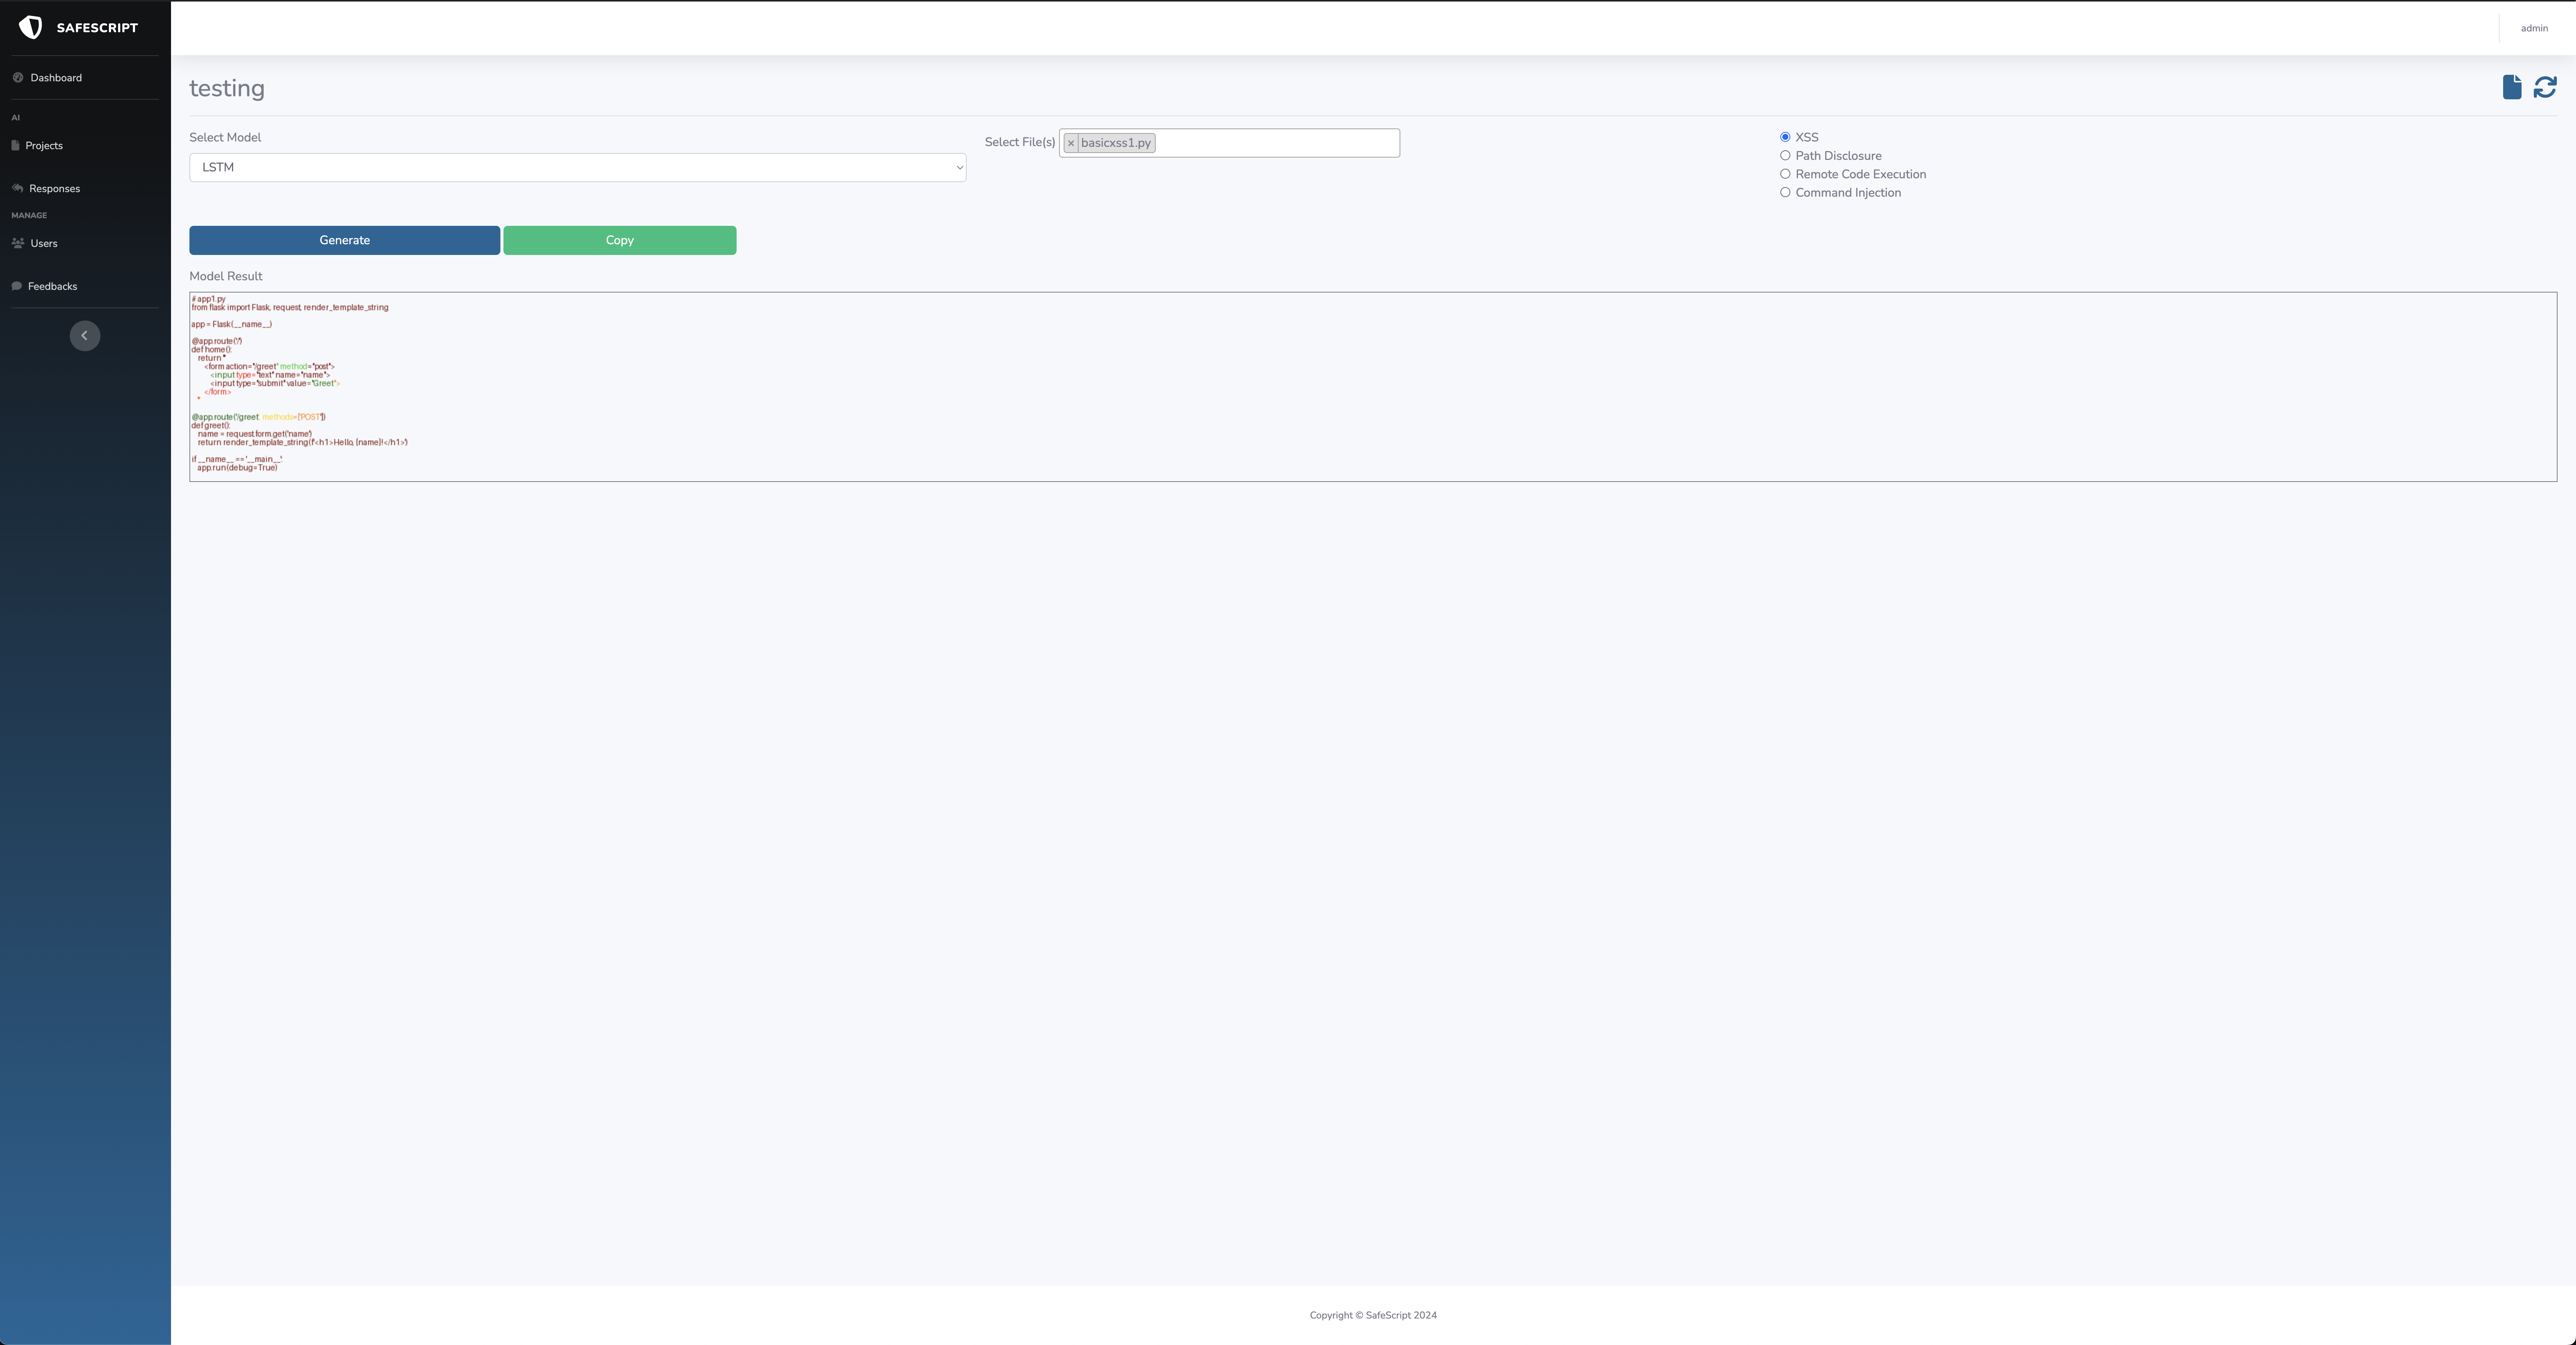
\includegraphics[width=0.6\linewidth]{images/xss1.png}
        \caption{Testing XSS vulnerability over LSTM model}
        \label{img:xss1}
    \end{figure}

    % Remote code execution
    \item Second case: The figure \ref{img:rce1} shows simple program from Flask.
    \begin{figure}[H]
        \centering
        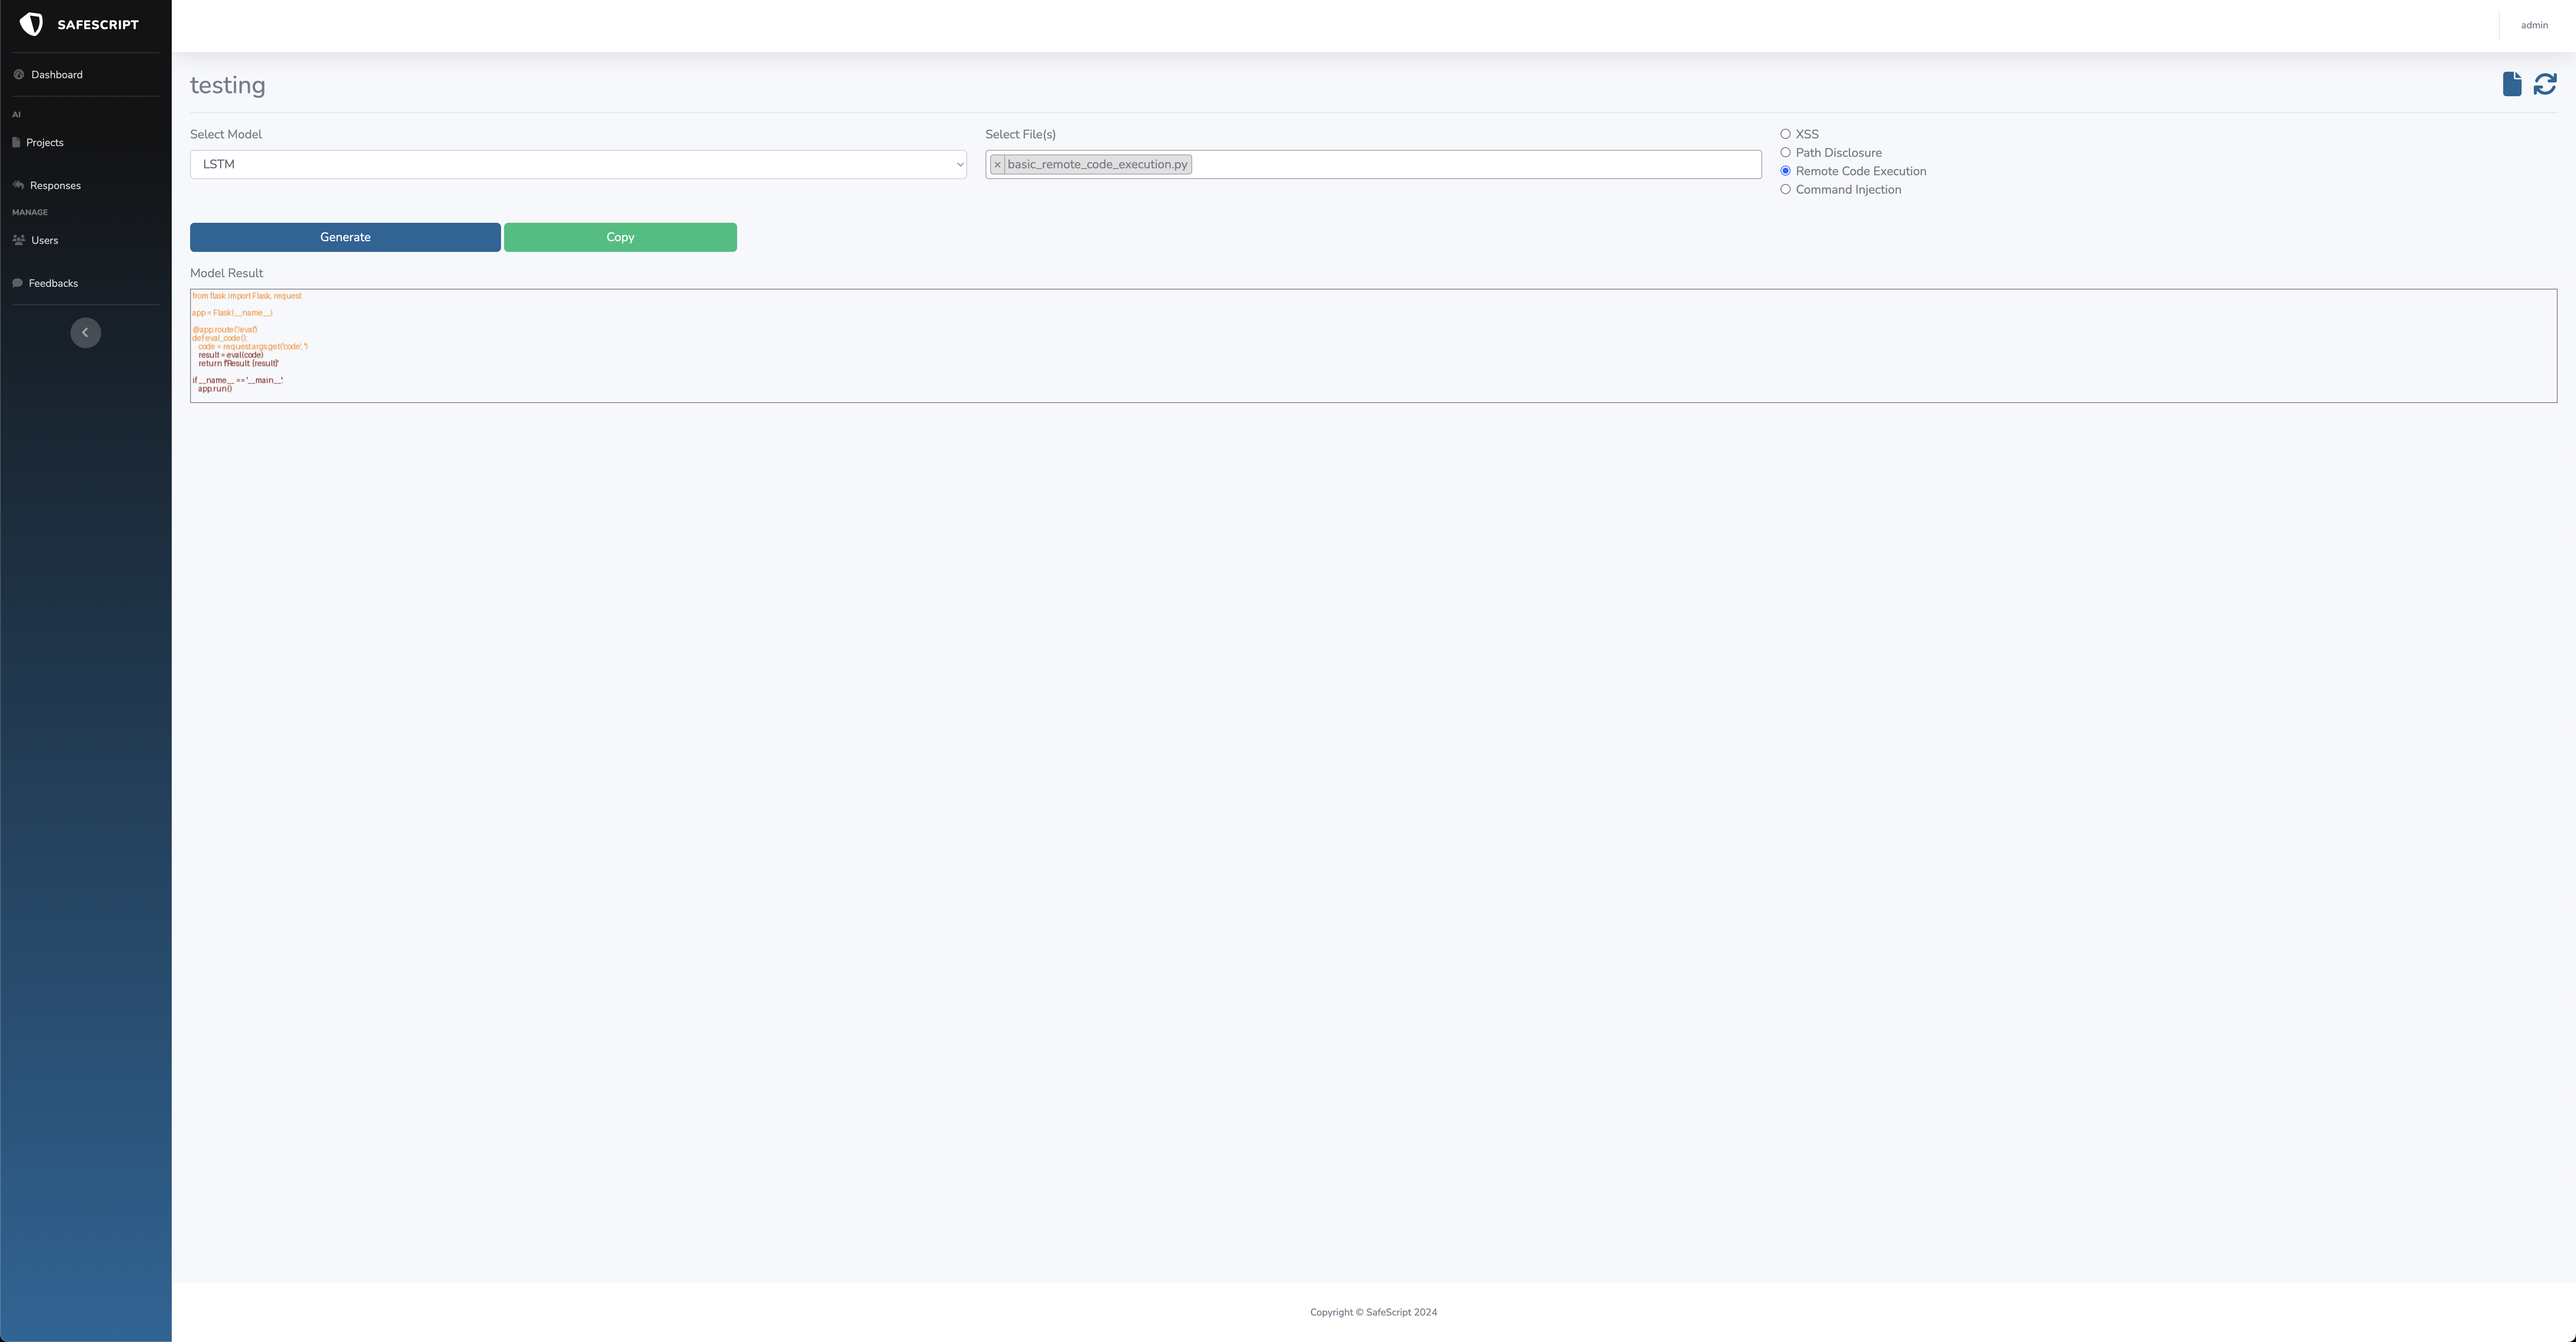
\includegraphics[width=0.6\linewidth]{images/rce1.png}
        \caption{Testing Remote Code Execution vulnerability over LSTM model}
        \label{img:rce1}
    \end{figure}

    % command injection
    \item Third case: The figure \ref{img:ci1} shows simple program from Flask.
    \begin{figure}[H]
        \centering
        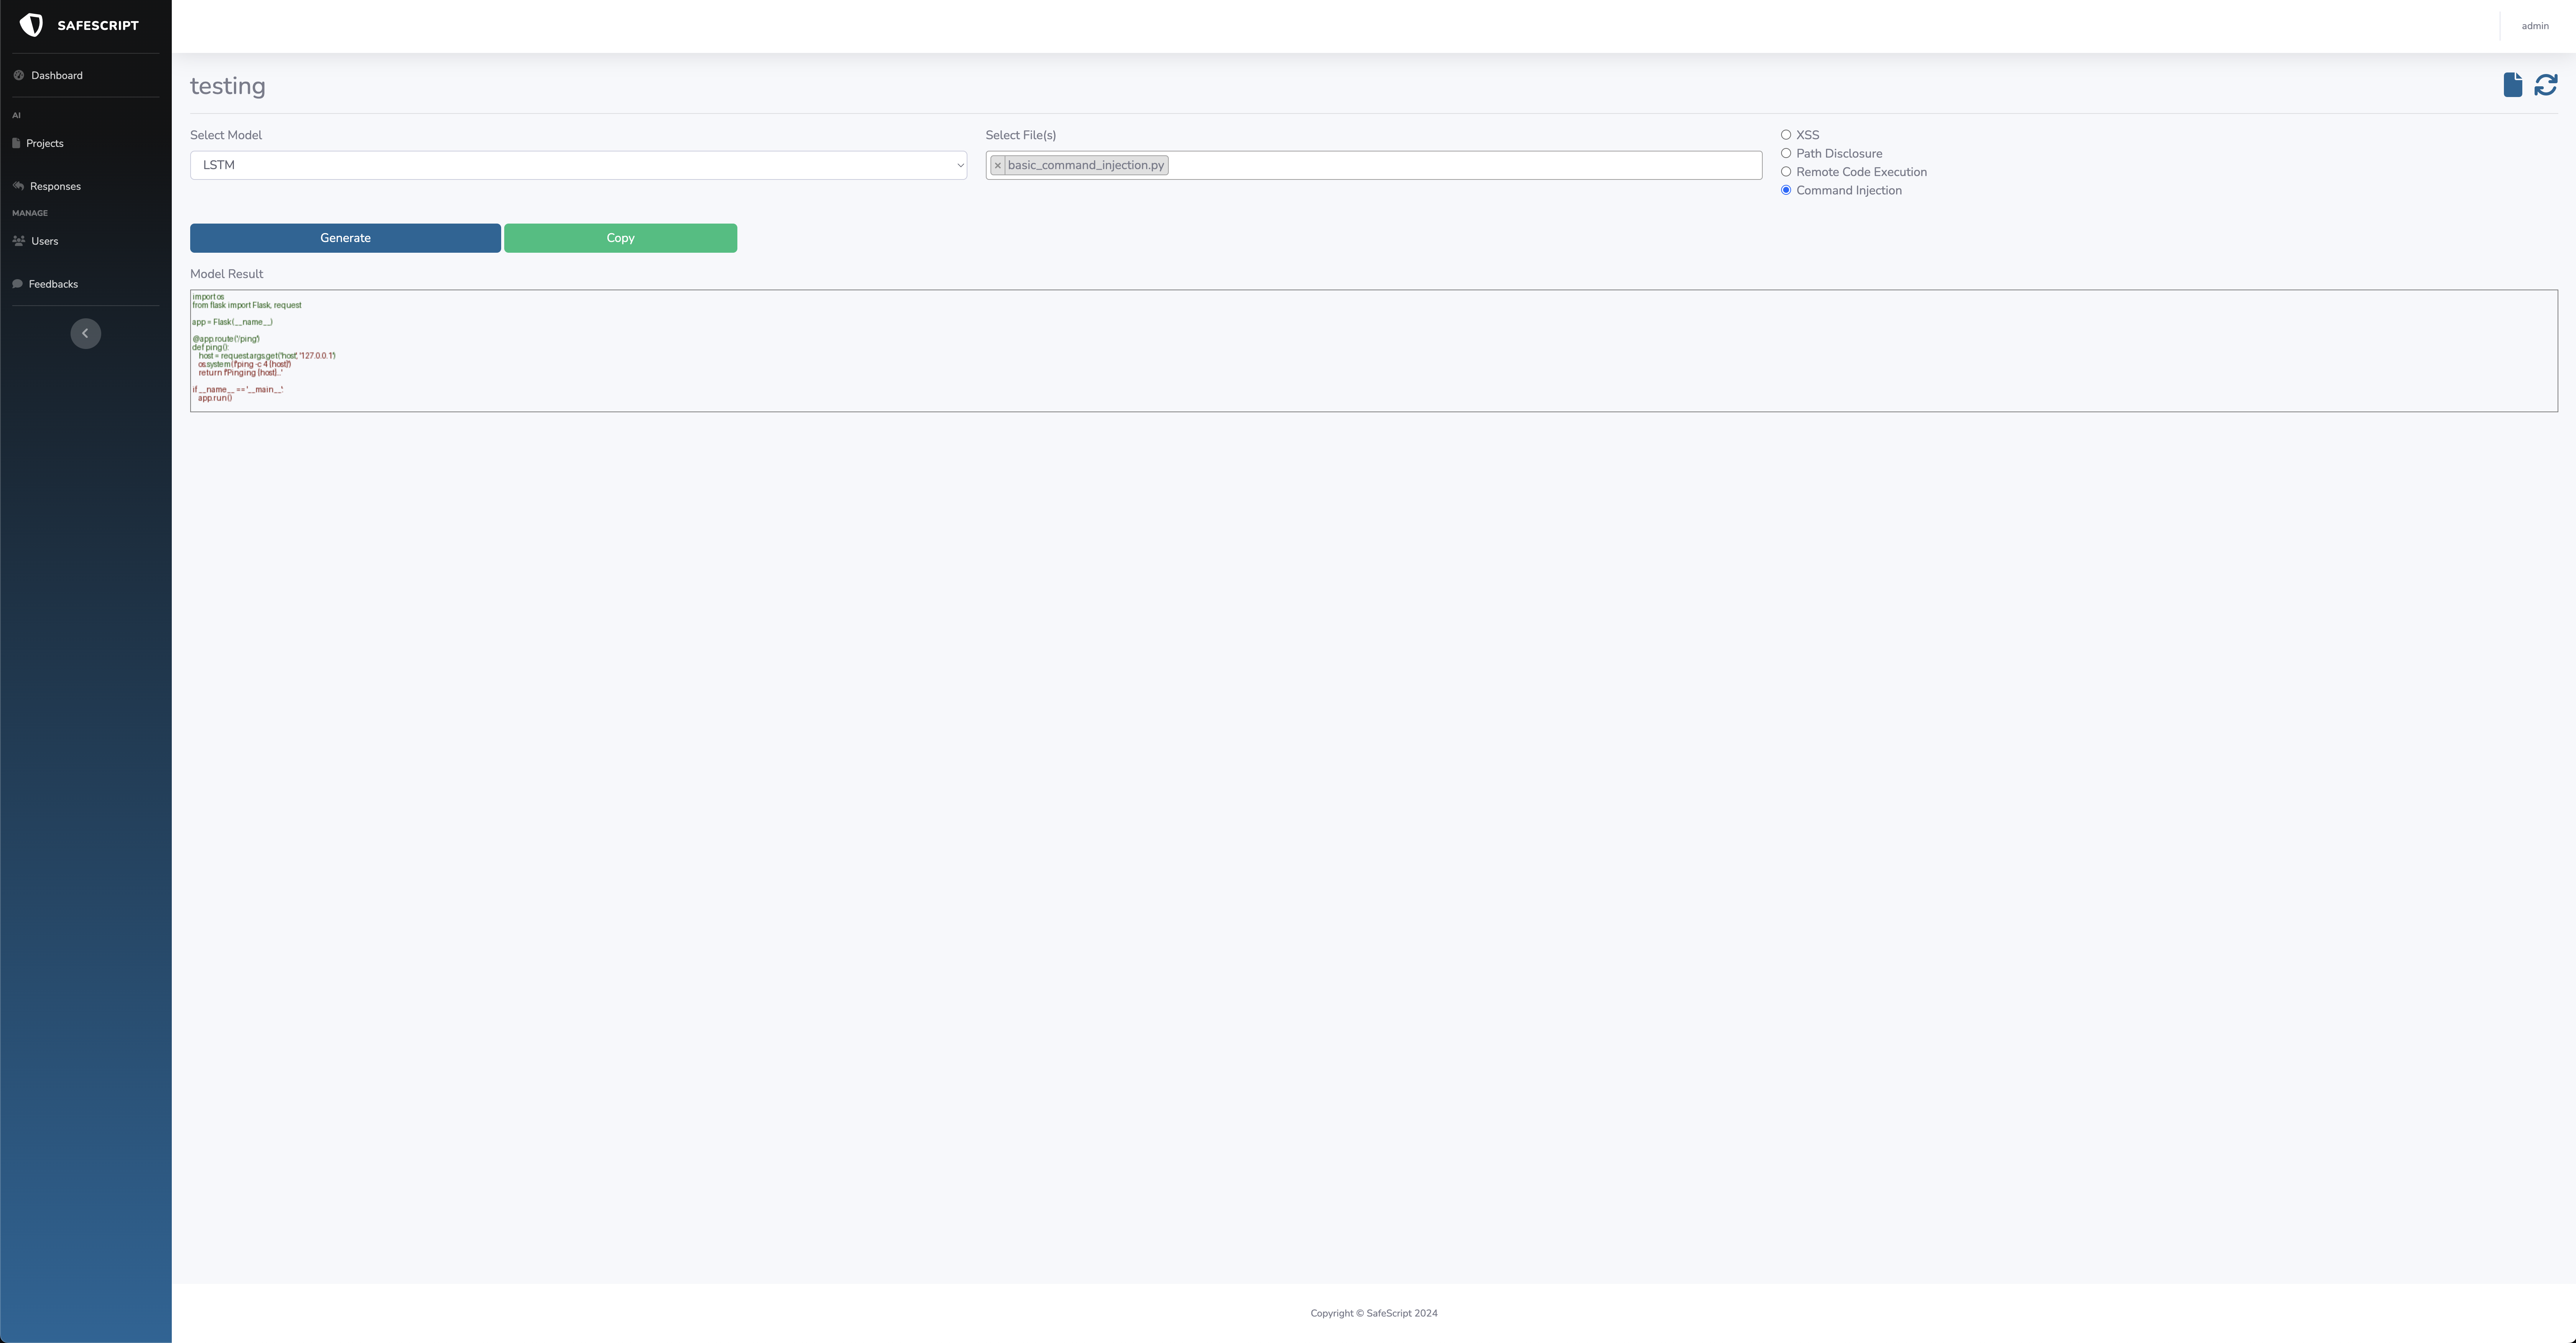
\includegraphics[width=0.6\linewidth]{images/ci1.png}
        \caption{Testing Command Injection vulnerability over LSTM model}
        \label{img:ci1}
    \end{figure}

    \item Fourth case: The figure \ref{img:pd1} shows simple program from Flask.
    \begin{figure}[H]
        \centering
        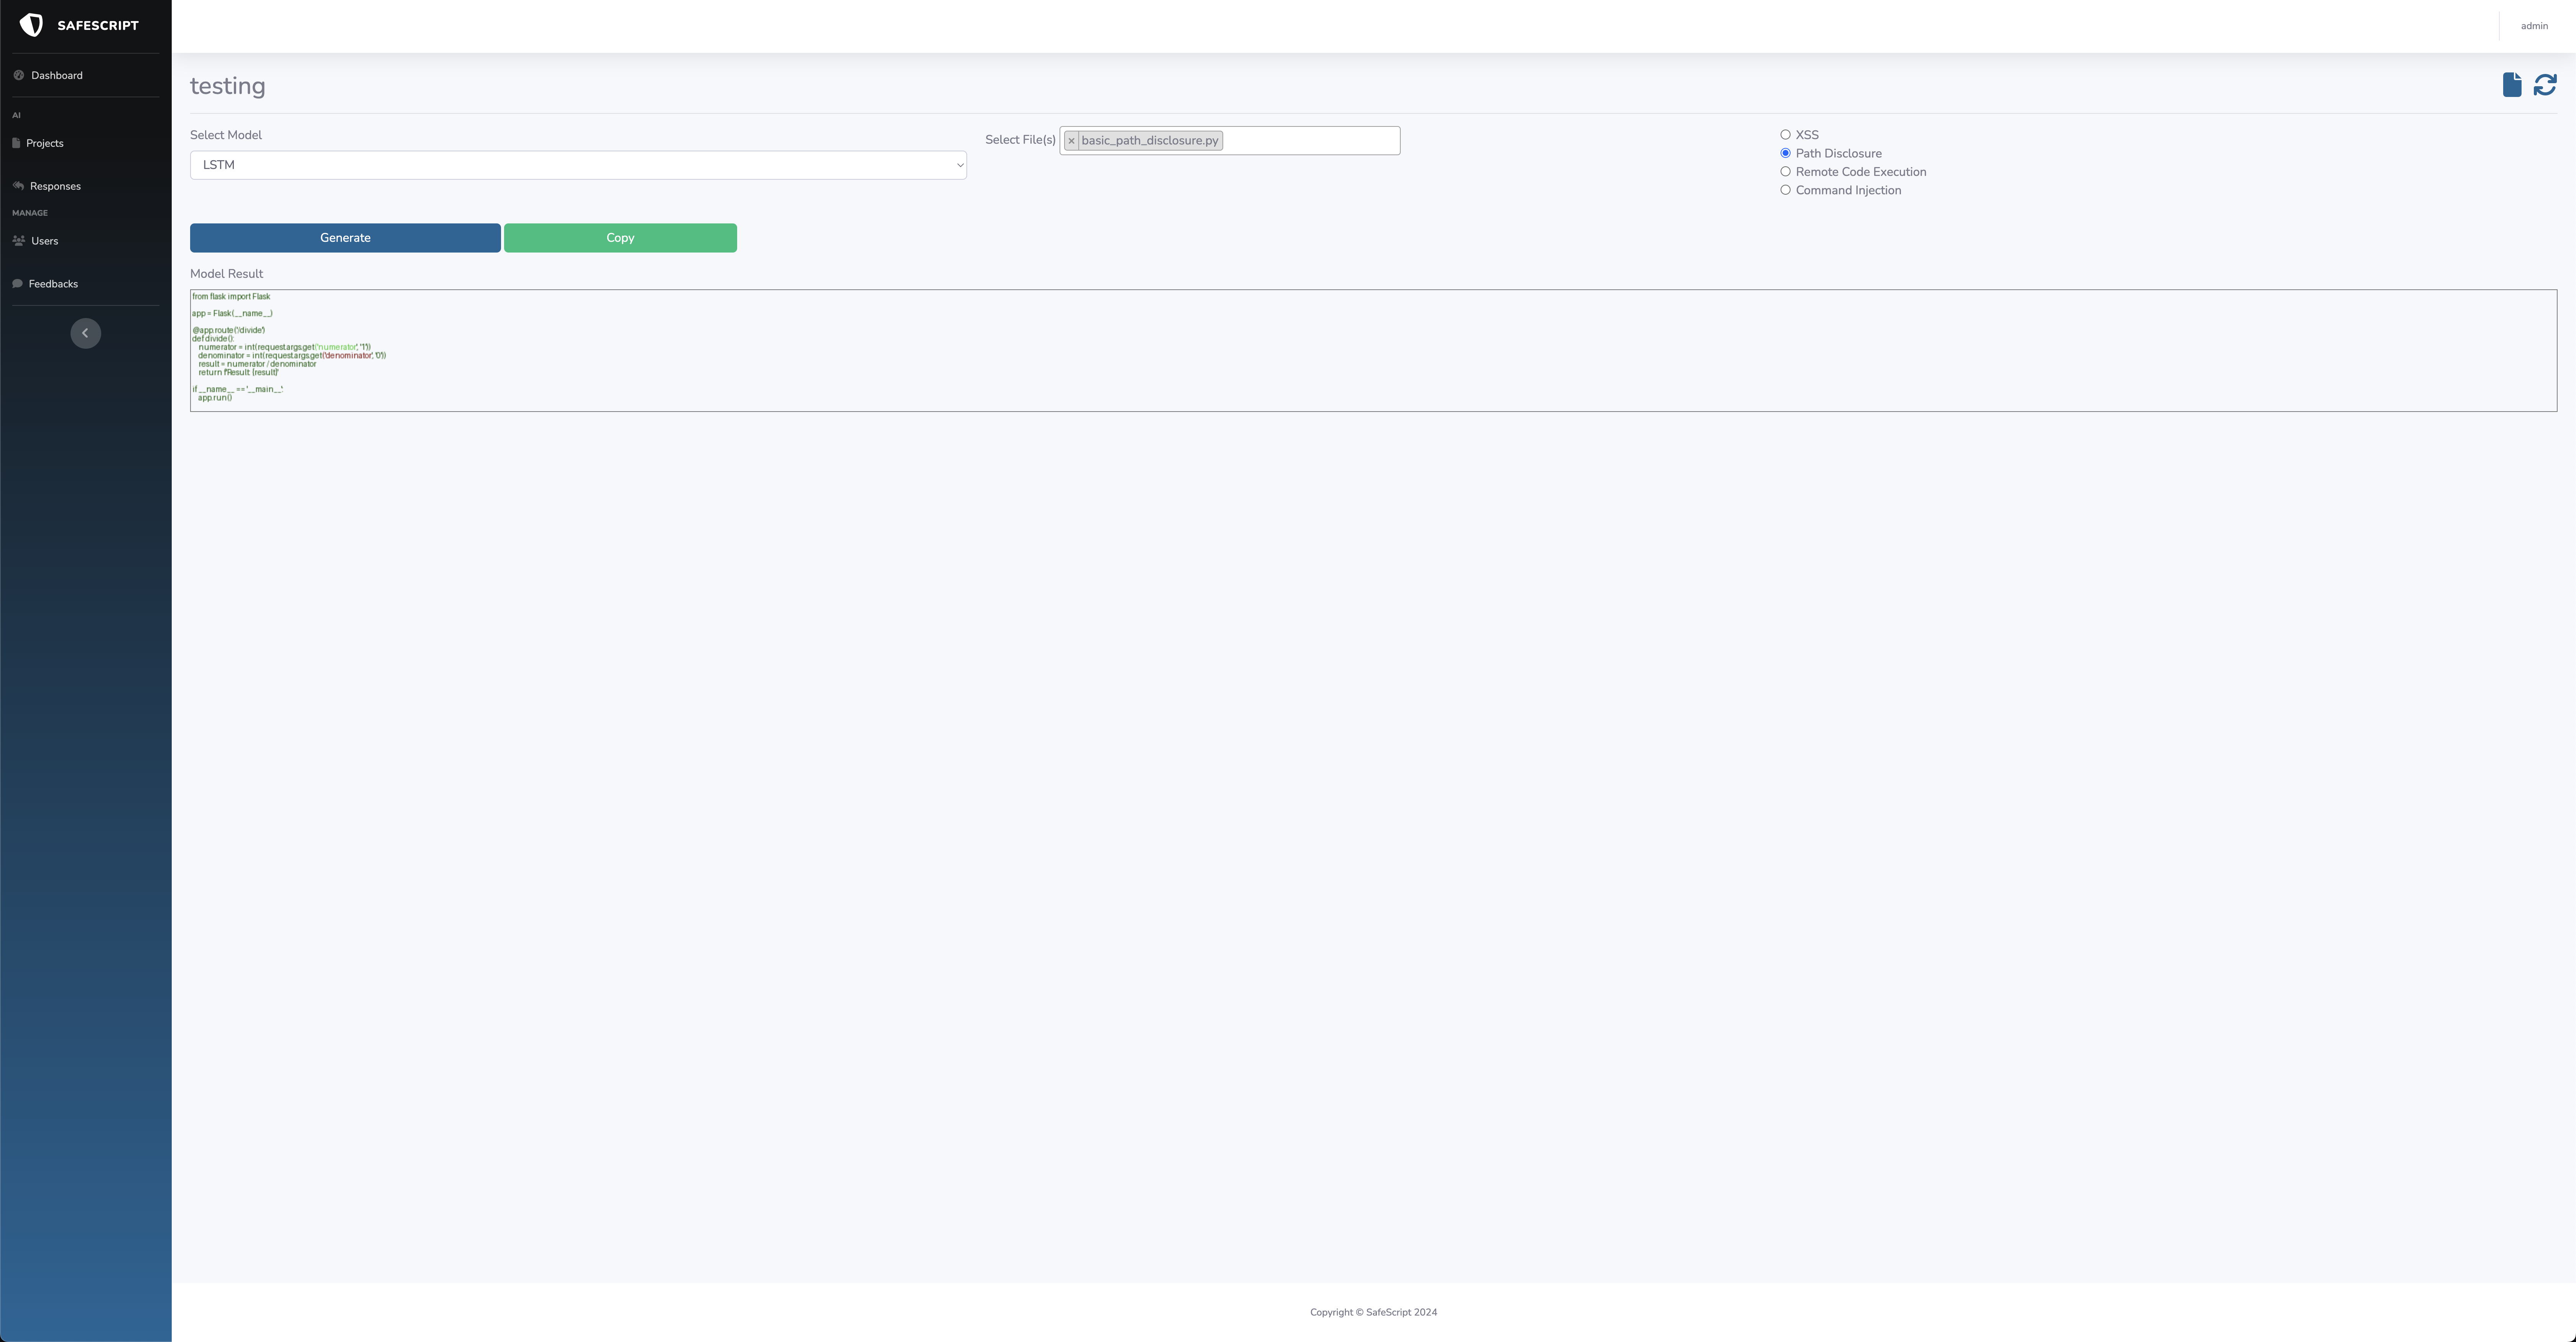
\includegraphics[width=0.6\linewidth]{images/pd1.png}
        \caption{Testing Path Disclosure vulnerability over LSTM model}
        \label{img:pd1}
    \end{figure}

\end{itemize}